\section{Introduction To Supervised Learning}
\subsection{Basic Concepts}
We use $\mathcal{X}$ and $\mathcal{Y}$ to denote the input space and the output space, where typically we have $\mathcal{X}=\mathbb{R}^p$, $\mathcal{Y}=\mathbb{R}$ or $\{0,1\}$. Let $(X,Y)$ be a pair of random variables distributed according to $F_{X,Y}$ which is a joint probability distribution on $\mathcal{X}\times\mathcal{Y}$.   

This means that: we have two measurable functions
\begin{equation}
\label{eq:3}
X: \Omega\mapsto \mathcal X  
\end{equation}
and
\begin{equation}
\label{eq:4}
Y: \Omega\mapsto \mathcal Y  
\end{equation}
The distribution of $X$:
\begin{equation}
\label{eq:1}
F_X(x)=P(\omega\in\Omega: X(\omega)\le x) =\int_{y\le x}f_X(y) dy  
\end{equation}
The joint distribution 
\begin{equation}
\label{eq:2}
F_{X,Y}(x,y)=P(\omega\in\Omega: (X(\omega),Y(\omega))\le (x,y)) 
=\int_{(u,v)\le (x,y)}f_{X,Y}(u,v) du\;dv
\end{equation}
and 
\begin{equation}
(X,Y): \Omega\mapsto \mathcal X\times \mathcal Y.
\end{equation}
\begin{equation}
(X,Y)(\omega) = (X(\omega), Y(\omega)) \in \mathcal{X}\times\mathcal{Y}
\end{equation}
then the probability of $(X,Y)$ in a measurable set of $\mathcal{X}\times\mathcal{Y}$, for example $M_1\times M_2$, can be written as
\begin{equation}
P(\omega\in\Omega: (X,Y)(\omega) \in M_1\times M_2)= P\left( \{\omega\in\Omega: X(\omega)\in M_1\} \cap \{\omega\in\Omega: Y(\omega)\in M_2\} \right)
\end{equation}
which is also equal to
\begin{equation}
\int_{M_1\times M_2} f_{X,Y}(u,v)dudv
\end{equation}

We can identify the distribution with its density function $f_{X,Y}(x,y)$. Usually the upper case $(X,Y)$ denotes random variables and the lower case $(x,y)$ denotes one specific sample. (where $x \in \mathcal{X}$ and $y \in \mathcal{Y}$).

\noindent We use $F_X$ and $F_{Y|X}$ to denote the marginal distribution of X and the conditional distribution of $Y$ given $X$. We also use $f_X(x)$ and $f_Y(y|X=x)$ to denote the marginal density function of $X$ and the conditional density function of $Y$ given $X=x$.\\
where the marginal density function of $X$ can be written as 
\begin{equation}
f_X(x)= \int_\mathcal{Y}f_{X,Y}(x,y) dy
\end{equation}
Actually, it is the same $f_X(x)$ given in (1.3), Because the RHS satisfies the definition of density function of $X$:
\begin{align}
\int_{\tilde{x} \leq x}	\int_\mathcal{Y}f_{X,Y}(\tilde{x},y) dy d\tilde{x} &= \int_{(u,v)<(x,+\infty)} f_{X,Y}(u,v)dudv\\
&=P(\omega\in\Omega: (X(\omega),Y(\omega))<(x,+\infty))\\
&=P(\omega\in\Omega: X(\omega)<x)\\
&=F_X(x)
\end{align}
Or you could view it as a simple proof of the equation(1.9).\\

And the conditional density function of $Y$ given $X=x$ can be written as
\begin{equation}
f_Y(y|X=x)= \frac{f_{X,Y}(x,y)}{f_X(x)}
\end{equation}
then the probability of $Y$ in a measurable set of $\mathcal{Y}$ when given $X=x$ can be computed as
\begin{equation}
P(Y \in M|X=x)= \int_{y\in M} \frac{f_{X,Y}(x,y)}{f_X(x)} dy
\end{equation}
For a particular case, if the conditional distribution of $Y|X$ is discrete, which means $Y$ takes value from a countable (or finite) set $\{y_1,...,y_n,...\}$ with probablity $p_1,...,p_n,...$ respectively. Of course we have $\sum_{i=1}^{\infty}p_i=1$, Then the probability is simpliy denoted by:
\begin{equation}
P(y_i|X=x)=P(y_i|x)=p_i
\end{equation}
We can see that the density function of pair $(X,Y)$ is uniquely identified by the marginal density function of $X$ and the conditional density function of $Y$ given $X=x$ for all $x \in \mathcal{X}$. So that $F_{X,Y}$ is uniquely identified by $F_X$ and $F_{Y|X}$. This provides another view of a sample $(x,y)$ drawn from the joint distribution $F_{X,Y}$, that we can firstly get $x$ from the marginal distribution $F_X$ and then get the corresponding label $y$ from the conditional distribution $F_{Y|X}$ given $X=x$.\\

\hrule 
\noindent Let $S = \{(x_1,y_1),...,(x_n,y_n) \}$ be an i.i.d. random
sample from $F_{X,Y}$. 
\hrule 

Let us put this more mathematically. Now we have a pair random variable $(X,Y)$, but we are supposed to draw samples from the joint distribution n times independently. To finish it, we have to introduce more random variables and make them independent and identically distributed(i.i.d.). We define:
\begin{equation}
Z=((X_1,Y_1), (X_2,Y_2),..., (X_n,Y_n)) :\Omega^n \mapsto (\mathcal{X}\times\mathcal{Y})^n	
\end{equation}
\begin{equation}
(\omega_1, \omega_2,..., \omega_n) \mapsto ((X,Y)(\omega_1), (X,Y)(\omega_2),..., (X,Y)(\omega_n))
\end{equation}
then for any $i$, $(X_i,Y_i)$ is the composition of the joint measurable function $Z$ and a projection $p_i$ from $(\mathcal{X}\times\mathcal{Y})^n$ to its i-th component:
\begin{equation}
(X_i,Y_i)=p_i \circ Z :\Omega^n \mapsto (\mathcal{X}\times\mathcal{Y})
\end{equation}
\begin{equation}
(X_i,Y_i)(\omega_1, \omega_2,..., \omega_n)= (X,Y)(\omega_i)
\end{equation}
It is easy to check these n-tuple random variables are i.i.d. We will show a simple explanation of the independence. Assume that $M_1, M_2,..., M_n$ are n measurable set of $\mathcal{X}\times\mathcal{Y}$, $M=M_1\times M_2\times...\times M_n$ and $\omega=(\omega_1, \omega_2,..., \omega_n)$, then
\begin{align}
P(\omega \in \Omega^n : Z(w)\in M) &= P((\omega_1, \omega_2,..., \omega_n)\in \Omega^n : (X,Y)(\omega_i) \in M_i, \forall 1\leq i \leq n ) \\
&= \prod_{i=1}^{n}P(\omega_i \in \Omega : (X,Y)(\omega_i) \in M_i) \\
&= \prod_{i=1}^{n}P(\omega \in \Omega^n : (X_i,Y_i)(\omega) \in M_i)
\end{align}
Which is obtained by  product measure of the product space $\Omega^n$. \\
\noindent Thus random variable $Z$ maps a event in $\Omega^n$ to a n-tuple samples $S = \{(x_1,y_1),...,(x_n,y_n) \}$.\\

\noindent The goal of supervised learning is to find a mapping $h:\mathcal{X}\mapsto\mathcal{Y}$  based on the dataset S, so that $h(X)$ is a good approximation of $Y$. When $\mathcal{Y}=\mathbb{R}$ the learning problem is often called regression and when $\mathcal{Y}=\{0,1\} or \{-1,1\}$, it is often called (binary) classification.\\

\begin{itemize}
	\item  For the classification problem, the conditional distribution $F_{Y|X}$ is just a distribution on $\{0,1\}$ which is determined by the conditional probability $p=P(Y=0|X=x)$ and $q=P(Y=1|X=x)$. ($p+q=1$)
	\item  For the regression problem, the conditional distribution $F_{Y|X}$ is a distribution over $\mathbb{R}$ which is determined by the conditional density function $f_Y(y|X=x)$. And for any measurable set $A$ (in most case $A$ is just an interval) of $\mathbb{R}$, the conditional probability is given by 
	$$P(Y \in A|X=x)= \int_{y\in A}f_Y(y|X=x)dy$$
\end{itemize}

\noindent The dataset S is often called the training set (or training data), and it is important since the distribution $F_{X,Y}$ is usually unknown. A learning algorithm is a procedure $\mathcal{A}$ which takes the training set S and procedures a predictor $\hat{h}=\mathcal{A}(S)$ as the output. Typically the learning algorithm will search over a space of functions $\mathcal{H}$, which we call the hypothesis space.\\
\begin{example}
	For a specific example, if we want the machine to recognize whether a picture is a cat or a dog.
	According to the results we want, we illustrate this problem with two models, using the classification method and the regression method respectively.\\
	
	Classification case: We just want the machine to give two answers, dog or cat. In this case, the sample we got has specific label says $(x,0)$ for dog or $(x,1)$ for cat. However, whether a picture is a cat or a dog is uncertain and subject to people's subjective consciousness. And that is exactly what the underlying conditional distribution explains. We can imagine $p=P(Y=0|X=x)$ represents the percentage of people who recognize the picture $x$ as a dog. Later we can see the optimal predictor will map the picture to a dog if $p>\frac{1}{2}$, to a cat if $p<\frac{1}{2}$. But we do not get the actual value of $p$. The regression model below can help to obtain the prediction of value of $p$.\\
	
	Regression case: We not only want the machine to give cat or dog answer, but also want it to give the probability of the given picture to be a cat or a dog. In this case the sample picture we got must has it probability label (i.e. a real number in $[0,1]$) represents the probability for this picture to be a dog. The conditional distribution gives no information since every picture has a specific probability. Actually this is the deterministic case we will talk in a short while.
\end{example}
\begin{example}
	\noindent For another specific example, if we want to use the pulse data of a woman to predict whether she is pregnant or not, the sample will be a pulse waveform. In oder to make the input space an Euclidean space, we discretized the time coordinates of the waveform. For example we get a wave for 10 seconds, we can divide it into 100 time-points, and then the y-axis value of these 100 points form a 100-dimension vector. Thus the input space $\mathcal{X}$ can be thought as $\mathbb{R}^{100}$. The output space $\mathcal{Y}$ is obviously $\{0,1\}$, where $1$ denotes pregnant and $0$ denotes not. Thus $\mathcal{X}\times\mathcal{Y}$ here is actually $\mathbb{R}^{100} \times \{0,1\}$. \\
	
	\noindent The basic hypothesis is that there is a distribution $F_{X,Y}$ on $\mathcal{X}\times\mathcal{Y}$,	 which means if we choose a random person and detect her pulse waveform, the discrete pulse data together with the pregnancy is considered as a joint random variable $(X,Y)$ whose distribution is $F_{X,Y}$. A sample drawn from $F_{X,Y}$ is a pair $(x,y)$, where $x$ is the wave data and y is the pregnancy or not. It is worth noting that, for the same wave data $x$, then $(x,0)$ and $(x,1)$ are both possible in our sample set. \\
	The marginal distribution of $X$ means we only consider the distribution of pulse data, ignoring the pregnancy. The marginal distribution of $Y$ means the probability of a woman getting pregnant, which has nothing to do with the pulse data. The conditional distribution of $Y|X=x$ indicates the probability to getting pregnant of a woman with specific pulse waveform $x$.
\end{example}

\subsection{Loss Function and Risk}
A loss function is a mapping $\ell:\mathcal{Y} \times \mathcal{Y}^* \mapsto \mathbb{R}^+$. For example, in binary classification the 0/1 loss function $\ell(y,p) = I(y\ne p)$ is often used and in regression the squared error loss function $\ell(y,p)=(y-p)^2$ is often used. Other loss functions include the following: absolute loss, Huber loss, $\epsilon-insensitive$ loss, hinge loss, logistic loss, exponential loss, modified least squares loss, etc. They will be discussed later in more details.

\noindent The performance of a predictor  $h:\mathcal{X}\mapsto\mathcal{Y}$ is measured by the expected loss, a.k.a. the risk or generalization error:
\begin{equation}
R(h): =\mathbb{E}_{X,Y}[\ell(Y, h(X))]
\end{equation}
where the expectation is taken with respect to the distribution $F_{X,Y}$. Since in practice we estimate $\hat{h}_S$ based on the training set S, we have $R(\hat{h}_S)$ itself a random variable. More precisely, $\mathcal{A}$ is a fucntion mapping $S$ to $\hat{h}_S$, then $R\circ \mathcal{A}$ maps $S$ to a real number, which is a function of random variable $S$. Thus we may also use the quantity $R(\mathcal{A})=\mathbb{E}_{S}[R(\hat{h}_S)]=\mathbb{E}_{S}[R\circ \mathcal{A}(S)]$
to characterize the generalization performance of the learning algorithm $\mathcal{A}$, which is also called the expected risk of the learning algorithm.\\

\noindent The risk is an important measure of the goodness of the predictor $h(.)$ since it tells how it performs on average in terms of the loss function $\ell(.,.)$ The minimum risk is defined as
\begin{equation}
R^*= \inf_h{R(h)}
\end{equation}
where the infimum is often taken with respect to all measurable functions. The performance of a given predictor/estimator can be evaluated by how close $R(h)$ is to $R^*$. Minimization of the risk is non-trivial because the underlying distribution $F_{X,Y}$ is in general unknown, and the training data S only gives us an incomplete knowledge of $F_{X,Y}$ in practice.

\subsection{Deterministic vs. stochastic(agnostic) scenarios}
When the label of a random variable $X$  can be uniquely determined by some measurable function $f: \mathcal{X} \to \mathcal{Y}$(with probability one), then the scenario is said to be deterministic. The "probability one" means that the graph of $f$, $\Gamma(f)=\{(x,y)\in \mathcal{X}\times \mathcal{Y}: y=f(x), x\in \mathcal{X}\}$ satisfies:
\begin{equation}
P(\omega \in \Omega: (X,Y)(\omega) \in \Gamma(f)) = 1
\end{equation}
Or more simply,
\begin{equation}
P(Y=f(X))=1
\end{equation}
In that case, it is suffices to consider a distribution $F$ over the input space $\mathcal{X}$ (instead of  $\mathcal{X}\times\mathcal{Y}$). The training sample is obtained by drawing $(x_1,..., x_m)$ according to $F$ and the labels are obtained via $f: y_i=f(x_i)$ for all $i \in [1, m]$. Many learning problems can be formulated within this deterministic scenario.\\

\noindent Within this setting, the output label is a deterministic function of the input, while in the stochastic case that is a probabilistic function of the input. More precisely, in the case $\mathcal{Y}=\mathbb{R}$ or $\{0,1\}$, there exsist a random variable $\xi$ and a deterministic function $f$ such that, $Y=f(X,\xi)$. It is easy to see that stochastic case is more general, and when the probability is one for each point in the input space, it becomes to the deterministic scenario.\\
For example, we can choose $\xi$ to be uniformly random on $[0,1]$. We will do that in the following two common cases.\\

\noindent In binary classification case , for a given $x \in \mathcal{X}$, the distribution over $\mathcal{Y}$ is determined by the probabilities $p(x)$ and $q(x)$, corresponding to the label $0$ and $1$. Then we can define $f$ to be,
\begin{numcases}{f(x,\xi)=}
0, & if 0 $\leq \xi < p(x)$ \\
1, & if $p(x) \leq \xi \leq 1$
\end{numcases}
In refression case, for a given $x \in \mathcal{X}$, the distribution over $\mathcal{Y}$ is determined by the conditional distributed function $F_{x}(y)$. Similarly we define $f$ to be,
\begin{equation}
f(x,\xi)= \inf\{y:F_x(y) \geq \xi\}
\end{equation}
Then for any fixed $x \in \mathcal{X}$, the distributed function of $f(x,\xi)$ is identical to that of $Y|X=x$.\\

\noindent By taking the expectation successively (which can be proved easily by $Fubini \ Theorem$) we have:
\begin{equation}
R(h)=\mathbb{E}_{X,Y}[\ell(Y, h(X))]=\mathbb{E}_{X} \left[ \mathbb{E}_{Y|X}[\ell(h(X),Y)] \right] 	
\end{equation}\\
In the deterministic case, the conditional distribution of $Y|X$ is only one possible value $f(X)$. Then $f$ is the target fouction we need to learn. Thus, the above becomes:
\begin{equation}
R(h)=\mathbb{E}_{X}[\ell(h(X),f(X))]
\end{equation}\\
\noindent An essential difference between these two scenarios is whether there exists a function with zero generalization error.
In the deterministic case, by definition, there exists a target function h with no generalization error: $R(h)=0$. In the stochastic case, generally there is a minimal non-zero error for any hypothesis, which says: $R^*>0$.\\
The arbitrariness of the loss function bring about this "generally". For example in the case $\mathcal{Y}=\mathcal{Y}^*=\mathbb{R}$, if we choose the loss function to be a strange one, $\ell(y,p)=|y-p|\exp(-|y-p|)$, which intends to make $\ell(y,p)$ decay to zero when the Euclidean distance of $x$ and $y$ increase to infinity. For this strange loss function, even in non-deterministic case, we can easily construct a series of $h_n$ such that $R(h_n)$ converge to zero, which means that $R^*=0$. \\

Fortunately, in binary classification or regression, if we choose the normal loss fucntion, $0/1$ error loss and squared error loss, then we can claim that a stochastic case is deterministic case if and only if $R^*=0$. \\

\noindent For the deterministic case, we have showed that $R^*=0$. To prove the other side, we need to prove that a stochastic case is deterministic case when $R^*=0$. Assume not, then there must exists a positive measure set $A\subseteq \mathcal{X}$, where the conditional distributution $Y|X=x$ is not concentrated in one value, which means for any $y\in \mathcal{Y}$, the probability $P(Y=y|X=x)\ne 1$.
That implies for any fixed $x\in A$, for any $y\in \mathcal{Y}$, we have
\begin{equation}
\mathbb{E}_{Y|X=x}[\ell(y,Y)]= \mathbb{E}_{Y|X=x}[(y-Y)^2]> 0
\end{equation}
We define a function $p(x)$ on $A$, (somewhere $p(x)$ can be $+\infty$)
\begin{equation}
p(x)= \inf_{y\in \mathcal{Y}} {E}_{Y|X=x}[(y-Y)^2]
\end{equation}
By the lemma in the next subsection, we know that $y=\mathbb{E}[Y|X=x]$ can achieve the infimum $\inf_{y\in \mathcal{Y}} {E}_{Y|X=x}[(y-Y)^2]$. So that $p(x)>0$ for any $x\in A$. 
Then for any measurable function $h: \mathcal{X} \to \mathcal{Y}$,
\begin{align}
R(h)&= \mathbb{E}_{X} \left[ \mathbb{E}_{Y|X}[\ell(h(X),Y)] \right]\\
&= \mathbb{E}_{X}[\mathbb{E}_{Y|X}[(h(X)-Y)^2]]\\
&\geq \mathbb{E}_{X}[p(x)]\\
&\geq \int_{x\in A} p(x) f_{X}(x) dx
\end{align}
Since $A$ is a set of positive measure, we can assume that $f_{X}(x)$ is positive almost everywhere on $A$. Together with the positiveness of $p(x)$, we have got the integration of a almost everywhere positve function on a positive measure set, which is postive for certain. Then $R(h)$ has a positive lower bound independent with $h$, which implies that $R^*>0$, a contradiction.\\
The smaller of $R^*$ means the more deterministic of the case.

\subsection{Binary Classification}
For classification problem, a predictor $h$ is also called a classifier, and the loss function for binary classification is often taken to be 0/1 loss. In this case, we have
\begin{equation}
R(h)=\mathbb{\mathbb{E}}_{X,Y}[\ell(Y,h(X))]=\mathbb{\mathbb{E}}_{X,Y}[I(Y\ne h(X))]=P(h(X)\ne Y)
\end{equation}

\noindent And the infimum risk $R^*$ is also known as the Bayes risk.\\
The following results show that the Bayes classifier, which is defined as 
\begin{equation}
h^*(x)=\arg\max_{y\in \{0,1\}}P(y|x)
\end{equation}
can achieve the Bayes risk.

\begin{lemma}
	Assume that $X$ is a random variable over $\mathbb{R}$. Define a function $f$ over $\mathbb{R}$, $f(\mu)= \mathbb{E}[(X-\mu)^2]$. If $E[|X|]=+\infty$, then $f(\mu)$ will be $+\infty$ everywhere on $\mathbb{R}$. If $E[|X|]<\infty$, then we know that $f$ is a quadratic function, which minimizes at $\mathbb{E}[X]$.
	$$\mathbb{E}[X]= \arg\min_{\mu \in \mathbb{R}} \mathbb{E}[(X-\mu)^2] $$
\end{lemma}
\begin{proof}
	If $E[|X|]=+\infty$, which means:
	\begin{equation}
	\int_{\mathbb{R}} |x|f_{X}(x) dx =+\infty
	\end{equation}
	For any $\mu \in \mathbb{R}$, there must exist a positive $a$, such that $(x-\mu)^2>|x|$ on $(-\infty,-a)\cup (a,+\infty)$. Then we have
	\begin{equation}
	\int_{\mathbb{R}} (x-\mu)^2f_{X}(x) dx \geq \int_{\mathbb{R}\backslash[-a,a]} |x|f_{X}(x) dx \geq +\infty
	\end{equation}
	Thus $E[(X-\mu)^2]=+\infty$ for any $\mu \in \mathbb{R}$.\\
	
	\noindent If $E[|X|]<+\infty$,
	\begin{align}
	f(\mu)&= \mathbb{E}[(X-\mu)^2]= \mathbb{E}[X^2-2\mu X+\mu^2]= \mu^2 -2\mathbb{E}[X]\mu +\mathbb{E}[X^2]\\
	&=(\mu -\mathbb{E}[X])^2 + \mathbb{E}[X^2] - (\mathbb{E}[X])^2
	\end{align}
	Thus $f(\mu)$ is a quadratic function which minimizes at $\mathbb{E}[X]$, and when $\mu$ get closer to $\mathbb{E}[X]$, $f(\mu)$ gets smaller.
\end{proof}

We can already draw some conclusions from this lemma. If we choose the loss function to be the squared error loss, $\ell(p,y)=(p-y)^2$, then generalization error becomes:
\begin{equation}
R(h)= \mathbb{E}_{X,Y}[(Y-h(X))^2] = \mathbb{E}_{X}[\mathbb{E}_{Y|X}[(Y-h(X))^2]]
\end{equation}
The lemma implies that $R(h)$ is minimized when $h(x)$ is nearest to $\mathbb{E}[Y|X=x]$ for every $x\in \mathcal{X}$, which means that $\big|h(x)-\mathbb{E}[Y|X=x]\big|$ should achieve its minial value.\\

Since 0/1 error loss is a special case of the squared error loss (restrict squared loss on $\{0,1\}$), we can apply the lemma to binary classification case. For binary classification, $\mathbb{E}[Y|X=x]= P(1|x)$. So that to minimize $R(h)$, $h(x)$ should be $1$ if $P(1|x)>\frac{1}{2}$, should be $0$ if $P(1|x)<\frac{1}{2}$. That is no other than $h^*(x)$.
\begin{corollary}
	For any classifier h we have $R(h) \geq R(h^*)$, i.e. $R(h^*)=R^*$
\end{corollary}

\subsection{Regression}
In regression we typically have $\mathcal{X}=\mathbb{R}^p$ and $\mathcal{Y}=\mathbb{R}$. And the risk is often measured by the squared error loss, $\ell(p,y)=(p-y)^2$. The following result shows that for squared error regression, the optimal predictor is the conditional mean function $\mathbb{E}[Y|X=x]$.
\begin{corollary}
	Suppose the loss function $\ell(.,.)$ is the squared error loss. Let $h^*(x) = \mathbb{\mathbb{E}}[Y|X=x]$, then we have $R(h^*)=R^*$.
\end{corollary}

\noindent Thus regression with squared error can be thought as trying to estimate the conditional mean function.
\subsection{Approximation Error vs. Estimation Error}
Suppose that the learning algorithm chooses the predictor from the hypothesis space $\mathcal{H}$, and define
\begin{equation}
h^*=\arg\inf_{h \in \mathcal{H}} R(h)
\end{equation}
i.e. $h^*$ is the best predictor among $\mathcal{H}$. Then the excess risk of the output $\hat{h}_S$ of the learning algorithm is
defined and can be decomposed as follows:
\begin{equation}
R(\hat{h}_S)-R^* = \underbrace{\left( R(h^*)-R^* \right)}_{approximation\ error} + \underbrace{\left( R(\hat{h}_S)-R(h^*) \right)}_{estimation\ error}
\end{equation}
Such a decomposition reflects a trade-off similar to the bias-variance tradeoff(maybe slightly more general). The approximation error is deterministic and is caused by the restriction of using $\mathcal{H}$. The estimation error is caused by the usage of a finite sample that cannot completely represent the underlying distribution.\\

\noindent The approximation error term behaves like a bias square term, and the estimation error behaves like the variance term in standard statistical estimation problems. Similar to the bias-variance trade-off, there is also a trade-off between the approximation error and the estimation error. Basically if $\mathcal{H}$ is large then we have a small approximation error but a relatively large estimation error and vice versa.

\section{Risk Minimization}
\subsection{Empirical risk Minimization}
Given a loss function $\ell$(.,.), the risk $R(h)$ is not computable as $F_{X,Y}$ is unknown. Thus we may not able to directly minimize $R(h)$ to obtain some predictors. Fortunately we are provided with the training data
$S=\{(x_1,y_1),...,(x_n, y_n)\}$ which represents the underlying distribution $F_{X,Y}$.
Instead of minimizing $R(h)=\mathbb{E}_{X,Y}[\ell(h(X),Y)]$, one may replace $F_{X,Y}$ by its empirical distribution and thus obtain the following minimization problem:
\begin{equation}
\hat{h}_S = \arg\min_{h \in \mathcal{H}} \frac{1}{m} \sum_{i=1}^{m}{\ell(h(x_i),y_i)}
\end{equation}
which we call empirical risk minimization(ERM). Furthermore, we also define the empirical risk $\hat{R}_S(h)$ as
\begin{equation}
\hat{R}_S(h):= \frac{1}{m} \sum_{i=1}^{m}{\ell(h(x_i),y_i)}
\end{equation}

\noindent We can already note that for a fixed $h \in \mathcal{H}$, the expectation of the empirical error based on an i.i.d. sample S is equal to the generalization error:
\begin{equation}
\mathbb{E}_{S\sim {D^m}}[\hat{R}_S(h)]=R(h)
\end{equation}
Indeed, by the linearity of the expectation and the fact that the sample is drawn i.i.d.,we can write
\begin{equation}
\mathbb{E}_{S\sim {D^m}}[\hat{R}_S(h)] = \frac{1}{m}\sum_{i=1}^{m}\mathbb{E}_{S\sim {D^m}}[{\ell(h(x_i),y_i)}] = \frac{1}{m}\sum_{i=1}^{m}\mathbb{E}_{S\sim{D^m}}[{\ell(h(x),y)}]
\end{equation}
for any $(x,y)$ in sample S. Thus,
\begin{equation}
\mathbb{E}_{S\sim {D^m}}[\hat{R}_S(h)] = \mathbb{E}_{S\sim{D^m}}[{\ell(h(x),y)}]= \mathbb{E}_{S\sim{D}}[{\ell(h(x),y)}]=R(h)
\end{equation}

\noindent Because under some conditions ( such as the expectation $R(h) < \infty $)\\  $\hat{R}_S(h) \xrightarrow{a.s.} R(h)$ by the law of large numbers, the usage of ERM is at least partially justified.\\

\noindent ERM covers many popular methods and is widely used in practice. For example, if we take $\mathcal{H} = \{h(x) | h(x)=\theta^Tx, \forall \theta \in \mathbb{R}^p\}$ and $\ell(y,p) = (y-p)^2$, then ERM becomes the well-known least squares estimation.
The celebrated maximum likelihood estimation (MLE) is also a special case of ERM where the loss function
is taken to be the negative log-likelihood function. Example: in binary classification $(x_1, y_1),..., (x_m,y_m)$
where $y_i \in (-1, 1)$ and $\mathcal{H} = \{h(x) | h(x)=\theta^Tx, \forall \theta \in \mathbb{R}^p\}$, the logistic regression is computed by minimizing the logistic loss
\begin{equation}
\hat{\theta} = \arg\min{\frac{1}{m}} \sum_{i=1}^{m}\log(1+\exp(-y_i\theta^T x_i))
\end{equation}
which is equivalent to MLE.

\subsection{Overfitting}
ERM works by minimizing the empirical risk $\hat{R}_S(h)$, while the goal of learning is to obtain a predictor with
a small risk $R(h)$. Although under certain conditions the former will converge to the latter as $n \rightarrow \infty$,
in practice we always have a finite sample and as a result, there might be a large discrepancy between those
two targets, especially when $\mathcal{H}$ is large and n is small. Overfitting refers to the situation where we have a
small empirical risk but still a relatively large true risk.\\
Consider the following example. Let $\ell(y, p)=(y-p)^2$ and we obtain the predictor $h$ by ERM:
\begin{equation}
\hat{h}_S = \arg\min_{h \in \mathcal{H}} \frac{1}{m} \sum_{i=1}^{m}{(h(x_i)-y_i)^2}
\end{equation}
\begin{figure}[htbp]
	\centering
	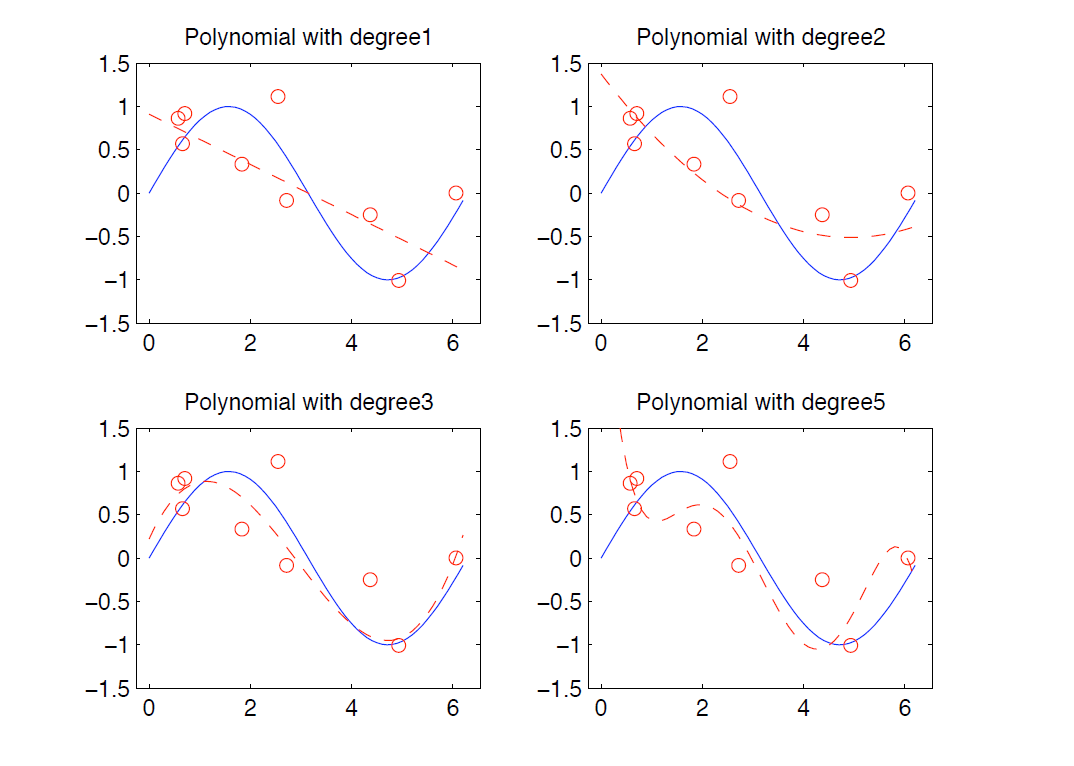
\includegraphics[width=1.1\linewidth]{6DL/figures/overfitting.png}
	\caption{Overfitting}
	\label{Overfitting1}
\end{figure}

\noindent Figure 1: Overfitting of polynomial regression. The true signal function(blue line) is $h^*(x)= sin(x)$, and
the function is fitted using 10 training examples (red dots). $P_1$ and $P_2$ show a lack of fitting(underfiting) and $P_5$ is overfitting.
\begin{figure}[htbp]
	\centering
	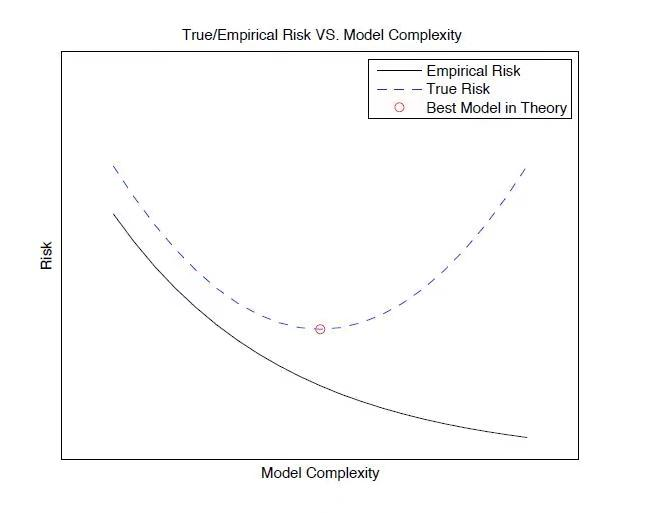
\includegraphics[width=0.8\linewidth]{6DL/figures/overfitting2.jpeg}
	\caption{True/empirical risk vs. model complexity}
	\label{Overfitting2}
\end{figure}

\noindent Figure1 shows the case where $\mathcal{H}$ is taken to be $P_1, P_2,...$, where $P_k$ is the set of all polynomial functions with order up to $k$\\

\noindent We can see that when $\mathcal{H}=P_3$ the fitted predictor will have a small risk(close to the true signal $sin(x)$)
Taking $P_k$ with larger k values as the hypothesis space can clearly improve its fitting with respect to the
10 observations(red dots), but this does not necessarily reduce the true risk as it overfits the training data.
Learning is more about generalization than memorization.

\subsection{Controlling Model Complexity}
Overfitting is mainly caused by the fact that the hypothesis space $\mathcal{H}$ is too large for the sample
Clearly the complexity of the hypothesis space $\mathcal{H}$ (i..e the size of $\mathcal{H}$) we can afford depends on the amount
of training data we have. For a given training dataset, the relationship between the true risk, the empirical
risk and model complexity can be best illustrated as in Figure 2.\\

\noindent One way to avoid overfitting is to choose $\mathcal{H}$ so that it is appropriate for the sample size. There are many ways to control the model complexity, and they are in fact quite similar in spirit. Here we list two commonly used approaches:\\

%\begin{adjustwidth}{1cm}{0cm}
\begin{enumerate}
	\item Take $\mathcal{H}_1$, $\mathcal{H}_2$, ..., $\mathcal{H}_n$,... to be a sequence of increasing sized spaces. For example, one typically has
	$\mathcal{H}_k \subset \mathcal{H}_{k+1}$ and $\cup \mathcal{H}_k= \mathcal{H}$. Given the training data S one finds $\hat{h}_S$ by minimizing
	\begin{equation}
	\hat{h}_{S,n} = \arg\min_{h \in \mathcal{H}_n} \hat{R}_S(h)
	\end{equation}
	This covers the method of Sieves and structural risk minimization (SRM) whoses hypothesis selected is the
	one among the $\hat{h}_{S,n}$ solutions with the smallest sum of the empirical error and a complexity term $complexity(\mathcal{H}_n,m)$ that depends on the size (or more generally the capacity, that is, another measure of the richness of $\mathcal{H}$) of $\mathcal{H}_n$, and the sample size $m$:
	\begin{equation}
	h^{SRM}_{S,n} = \arg\min_{h \in \mathcal{H}_n} \hat{R}_S(h)+complexity(\mathcal{H}_n,m)
	\end{equation}
	
	\item Define a penalty function $\Omega: \mathcal{H} \mapsto \mathbb{R}^+$ and find $\hat{h}_S$ by the following optimization procedure which is called regularization:
	\begin{equation}
	\hat{h}_S = \arg\min_{h \in \mathcal{H}} \hat{R}_S(h)+ \lambda \Omega(h)
	\end{equation}
	where $\lambda >0$ is a regularization, which can balances the trade-off between goodness-of-fit and model complexity. The regularization term $\Omega(h)$ is typically
	defined as $||h||^2$ for some norm $||.||$ when $\mathcal{H}$ is a vector space. In practice, $\lambda$
	is typically selected using n-fold cross-validation. This is also known as the penalized empirical risk minimization.\\
\end{enumerate}
%\end{adjustwidth}

\noindent In practice we often need to select $\mathcal{H}_n$ or $\lambda$ based on the training data to achieve a good balance between goodness-of-fit and model complexity.\\
\begin{example}
	\noindent Consider the following regression problem: let $\mathcal{H} = \{h(x) | h(x)=\theta^Tx, \forall \theta \in \mathbb{R}^p\}$ and we are trying to find an estimator $\hat{\theta}$ which minimizes the risk $\mathbb{E}_{X,Y}[(Y-\theta^TX)^2]$. For the first approach, we could define a sequence of increasing constants: $0\leq \eta_1 \leq ... \leq \eta_k \leq ...$, and define $\mathcal{H}_k = \{h(x) | h(x)=\theta^Tx, \theta^T\theta \leq \eta_k\}$. For the
	second approach we define $\Omega(h) = \theta^T\theta$. Then it is well-known from optimization that those two approaches
	become mathematically equivalent, i.e. for any $\eta_k$ there exists a $\lambda$ such that those two optimization problems
	have the same solution. The following shows a proof of the equivalence:\\
	
	\noindent For the second approach, we need to find the optimal $\bar{\theta}$ such that:
	\begin{equation}
	\bar{\theta} = \arg\min_{\theta \in \mathbb{R}^n}\frac{1}{m} \sum_{i=1}^{m} (\theta^Tx_i-y_i)^2+\lambda \theta^T\theta 
	\end{equation}
	
	where $\lambda$ is non-negative.\\
	
	Observe that the objective function is convex and a quadratic function, then it is a convex quadratic optimization problem with no constraint, so that $\bar{\theta}$ is the minimum solution if and only if:
	\begin{equation}
	\nabla_\theta (\frac{1}{m} \sum_{i=1}^{m}(\theta^Tx_i-y_i)^2+\lambda \theta^T\theta )|_{\bar {\theta}} = 0 
	\end{equation}\\
	
	\noindent For the first approach, we need to find the optimal $\bar{\theta}$ such that:
	\begin{equation}
	\bar{\theta} = \arg\min_{\theta \in X}\frac{1}{m} \sum_{i=1}^{m} (\theta^Tx_i-y_i)^2 
	\end{equation}
	
	where $X = \{\theta \in \mathbb{R}^n | \theta^T\theta \leq \eta_k \}$.
	Which is also a convex quadratic optimization problem with the feasible region $X$.
	The Lagrange funtion is defined as:
	\begin{equation}
	\mathcal{L}(\theta, \alpha) = \frac{1}{m} \sum_{i=1}^{m} (\theta^Tx_i-y_i)^2+\alpha (\theta^T\theta-\eta_k)	 
	\end{equation}
	
	For $\eta_k > 0$, $X$ is a closed ball whose interior $int(X) \ne \phi$. Then by the KKT conditions we know that the necessary and suficient condition of the constrained problem is: there exists $\bar{\alpha} \geq 0$ such that:
	\begin{align}
	&\nabla_\theta \mathcal{L}(\bar{\theta}, \bar{\alpha}) = 	\nabla_\theta (\frac{1}{m} \sum_{i=1}^{m}(\theta^Tx_i-y_i)^2+ \bar{\alpha} \theta^T\theta )|_{\hat{\theta}} = 0 \\ 
	&\nabla_\alpha \mathcal{L}(\bar{\theta}, \bar{\alpha}) = \bar{\theta}^T\bar{\theta}-\eta_k \leq 0 \\
	&\bar{\alpha} = 0 \ \ or \ \ \bar{\theta}^T\bar{\theta}  = \eta_k	      
	\end{align}
	When $\bar{\alpha} = 0$, that means the constraint condition $\theta^T\theta \leq \eta_k$ has no effect on the minimization problem. We will get the same minimal solution when $\theta$ runs over $\mathbb{R}^n$.\\
	When $\bar{\alpha} \ne 0$, that means $\bar{\theta}^T\bar{\theta}  = \eta_k$ and the minimal solution is obtained at the boundary of $X$.\\
	In both case, we take $\bar{\alpha}$ to be the penalty parameter $\lambda$ then (12) is equivalent to (15),(16),(17), and we have proved that the constrained problem is equivalent to a non-constrained problem with a penalty term adding to the objective funtion.
\end{example}
\section{Concentration Inequalities and PAC Learning}
\subsection{Generalization Error Bounds and PAC learning}
Although the concept of consistency of a learning algorithm is very important, it only measures how the expectation of a random variable $R(\hat{h}_S)$ converges to the optimal Bayes risk asymptotically. However, it does not say how fast this convergence is, and neither does it tell us how this random variable is distributed. In particular, we are interested in probability bounds of the generalization error, such as the following: "with
probability at least $1-\epsilon$, the risk $R(\hat{h}_S)$ is bounded by some quantity."\\
Recall that the excess risk can be decomposed into approximation error and estimation error, i.e.
\begin{equation}
R(\hat{h}_S)-R^* = \underbrace{\left( \inf_{h \in \mathcal{H}} R(h)-R^* \right)}_{approximation\ error} + \underbrace{\left( R(\hat{h}_S)-\inf_{h \in \mathcal{H}} R(h) \right)}_{estimation\ error}
\end{equation}
The approximation error is deterministic and mainly caused by two possible reasons: (1) the restriction
of using the function class $\mathcal{H}$; (2)if $\inf_{h \in \mathcal{H}} R(h)$ in the above equation were replaced by the minimum risk achievable by the learning algorithm with infinite amount of data, then it can also be caused by the systematic
as of the learning algorithm. Such an error is often not controllable as we do not know the underlying distribution $D_{X,Y}$. On the other hand, the estimation error depends on the sample size, the function class $\mathcal{H}$ and the learning algorithm which we have control over. We would like to obtain probability bounds for
the estimation error. The definition of agnostic PAC-learning is also based on the estimation error.\\

\noindent The following introduces the Probably Approximately Correct(PAC) learning framework. We denote by $O(n)$ an upper bound on the cost of the computational representation of any element $x \in \mathcal{X}$. For example, $x$ may be a vector in $\mathbb{R}^n$, for which the cost of an array-based representation would be in $O(n)$
\begin{definition}[Definition: Agnostic PAC-learning]
	Let $\mathcal{H}$ be a hypothesis set. $\mathcal{A}$ is an agnostic PAC-learning algorithm if there exists a polynomial function poly(.,. .,.,) such that for any $\epsilon > 0$ and $\delta > 0$, for all distributions $D$ over $\mathcal{X} \times \mathcal{Y}$, the following holds for any sample size $m \geq poly(1/\epsilon, 1/\delta, n)$:
	\begin{equation}
	P_{S \sim D^m} \left( R(h_S)-\inf_{h \in \mathcal{H}} R(h) \leq \epsilon \right) \geq 1-\delta
	\end{equation} 
\end{definition}

\noindent The probably approximately correct(PAC) learning model typically states as follows: we say that $\hat{h}_S$ is $\epsilon-accurate$ with probability $1-\delta$, if
In other words, we have $R(h_S)-\inf_{h \in \mathcal{H}} R(h) \leq \epsilon$ with probability at least $(1-\delta)$.\\

Specifically, if we use ERM to obtain our predictor $\hat{h}_S = \arg\min_{h \in \mathcal{H}} \hat{R}_S(h)$, and assume that $\inf_{h \in \mathcal{H}} R(h) = R(h^*)$ for some $h^* \in \mathcal{H}$, then we have:
\begin{align}
R(\hat{h}_S)-\inf_{h \in \mathcal{H}}R(h) &= R(\hat{h}_S)-\hat{R}_S(\hat{h}_S)+\hat{R}_S (\hat{h}_S)-R(h^*) \\
&\leq R(\hat{h}_S)-\hat{R}_S (\hat{h}_S)+\hat{R}_S (h^*)-R(h^*) \\
&\leq 2\sup_{h \in \mathcal{H}} |R(h)-\hat{R}_S (h)|	
\end{align}
Thus if we can obtain uniform bound of $\sup_{h \in \mathcal{H}} |R(h)-\hat{R}_S (h)|$ then the approximation error can be bounded.
Thus again justifies the usage of the ERM method.\\
Intuitively, for any $h \in \mathcal{H}$, $\hat{R}_S(h)$ is a random variable which follows a Binomial distribution with mean $R(h)$. Or we could think of it as the average of a series of random variables. Thus we should be
able to bound the difference between an average of a set of random variables and their mean. The uniform bound, however, will depend crucially on how large/complex the hypothesis space $\mathcal{H}$ is.\\

\subsection{Concentration Inequalities}
\begin{theorem}[Markov Inequality]
	For any nonnegative random variable X and $\epsilon > 0$,
	$$P(X \geq \epsilon) \leq \frac{\mathbb{E}[X]}{\epsilon}$$
\end{theorem}


\begin{theorem}[Chernoff Inequality]
	For any random variable X and $\epsilon > 0$,
	$$P(X \geq \epsilon) \leq \frac{\mathbb{E}[\exp(tX)]}{exp(t\epsilon)}$$
	and thus
	$$P(X \geq \epsilon) \leq \inf_{t > 0} \frac{\mathbb{E}[exp(tX)]}{\exp(t\epsilon)}$$
\end{theorem}

\begin{theorem}[Chebyshev Inequality]
	For any random variable X and $\epsilon > 0$,
	$$P(|X-\mathbb{E}[X]| > \epsilon) \leq \frac{\mathbb{V}[X]}{\epsilon^2}$$
\end{theorem}

\begin{lemma}
	If random variable X has mean zero, i.e. $\mathbb{E}[X]=0$, and is bounded in $[a,b]$, then for any $s > 0$,
	$$\mathbb{E}[\exp(sX)] \leq \exp(s^2(b-a)^2/8)$$
\end{lemma}

\begin{theorem}[Hoeffding Inequality]
	Let $X_1 ,..., X_m$ be independent bounded  random variables such that $X_i \in [a_i, b_i]$ with probability $1$. Let $S_m=\sum_{i=1}^{m} X_i$. Then for any $\epsilon > 0$, we have
	\begin{align}
	& P(S_m-\mathbb{E}[S_m] \geq \epsilon) \leq \exp \left(-\frac{2\epsilon^2}{\sum_{i=1}^{m}(b_i-a_i)^2} \right)\\
	& P(S_m-\mathbb{E}[S_m] \leq -\epsilon) \leq \exp \left(-\frac{2\epsilon^2}{\sum_{i=1}^{m}(b_i-a_i)^2} \right)\\
	& P(|S_m-\mathbb{E}[S_m]| \geq \epsilon) \leq 2\exp \left(-\frac{2\epsilon^2}{\sum_{i=1}^{m}(b_i-a_i)^2} \right)
	\end{align}	
\end{theorem}

\begin{theorem}[McDiarmid's Inequality]
	Let $X_1,...,X_m \in \mathcal{X}^m$ be a set of $m \geq 1$ independent random variables and assume that there exist $c_1,...,c_m > 0$ such that $f: \mathcal{X} \to \mathbb{R}$ satisfies the following conditions:
	$$|f(x_1,...,x_i,...,x_m)-f(x_1,...,x\prime_i,...,x_m)| \leq c_i$$
	for all $i \in [1,m]$ and any points $x_1,...,x_m,x\prime_i \in \mathcal{X}$. Let $f(S)$ denote $f(X_1,...,X_m)$, then for all $\epsilon > 0$, the following inequalities hold:
	\begin{align}
	& P(f(S)-\mathbb{E}[f(S)] \geq \epsilon) \leq \exp \left(-\frac{2\epsilon^2}{\sum_{i=1}^{m}c_i^2} \right)\\
	& P(f(S)-\mathbb{E}[f(S)] \leq -\epsilon) \leq \exp \left(-\frac{2\epsilon^2}{\sum_{i=1}^{m}c_i^2} \right)\\
	& P(|f(S)-\mathbb{E}[f(S)]| \geq \epsilon) \leq 2\exp \left(-\frac{2\epsilon^2}{\sum_{i=1}^{m}c_i^2} \right)
	\end{align}
\end{theorem}

\section{Empirical Risk vs True Risk}
As follows from the previous discussion, the technical results behind the PAC learning framework are bounds on the difference 
between the empirical and true risk which are uniform with respect to the element $h\in \mathcal{H}$, i.e. bounds on
\begin{equation}
\sup_{h\in \mathcal{H}} |\hat{R}(h) - R(h)|
\end{equation}
The quantity $\hat{R}(h)$ is a random variable, so we really need to consider
\begin{equation}
\mathbb{E}(\sup_{h\in \mathcal{H}} |\hat{R}(h) - R(h)|)
\end{equation}
and
\begin{equation}
\mathbb{P}(\sup_{h\in \mathcal{H}} |\hat{R}(h) - R(h)| \geq \epsilon)
\end{equation}
In particular, what we want is a bound of the form
\begin{equation}
\mathbb{P}(\sup_{h\in \mathcal{H}} |\hat{R}(h) - R(h)| \geq \epsilon) \leq C(\epsilon, m)
\end{equation}
where $m$ is the number of samples and the function $C(\epsilon, m)$ decays rapidly as $m\rightarrow \infty$.

\subsection{Guarantees for finite hypothesis sets-consistent case}
We say the hypothesis $h_S$ returned by the algorithm is consistent, if it admitts no error on
the training sample $S$. In this section, we present a general sample complexity
bound, or equivalently, a generalization bound, for consistent hypotheses, in the
case where the cardinality $\mathcal{H}$ of the hypothesis set is finite.
\begin{lemma}
	For the special case: $\mathcal{H} = \{h\}$, and $h$ is consistent with sample S, which means $\hat{R}_S (h)=0$, then we have:
	$$P \left( \hat{R}_S (h)=0, R(h) \geq \epsilon \right) \leq \exp(-m\epsilon)$$
\end{lemma}
\begin{proof}
	\begin{align}
	P \left( \hat{R}_S (h)=0, R(h) \geq \epsilon \right) &\leq P\left( \hat{R}_S (h)=0 \big| R(h) \geq \epsilon \right) \\
	&= (1-R(h))^m \big|_{R(h) \geq \epsilon} \\
	&\leq (1-\epsilon)^m \\
	&\leq \exp(-m\epsilon) 
	\end{align}
\end{proof}

\begin{theorem}[Learning bounds-Finite $\mathcal{H}$, consistent case]
	Let $\mathcal{H}$ be a finite set of functions mapping from $\mathcal{X}$ to $\{0,1\}$. Let $\mathcal{A}$ be an algorithm that for any target function $f \in \mathcal{H}$ and i.i.d. sample $S$ returns a consistent hypothesis $h_S$: $\hat{R}_S (h_S)=0$. Then for any $\epsilon, \delta > 0 $, the inequality $P_{S \sim D^m} (R(h_S) \leq \epsilon ) \geq 1-\delta$ holds if:
	\begin{equation}
	m \geq \frac{1}{\epsilon}(\log(|H|) + \log \frac{1}{\delta})
	\end{equation}
	This sample complexity result damits the following equivalent statement as a generalization bound: for any $\epsilon, \delta > 0 $, with probability at least $1-\delta$,
	\begin{equation}
	R(h_S) \leq \frac{1}{m} (\log(|H|) + \log \frac{1}{\delta})
	\end{equation}
\end{theorem}

\begin{proof}
	Fix $\epsilon > 0$. We do not know which consistent hypothesis $h_S \in \mathcal{H}$ is selected by the algorithm $\mathcal{A}$. This hypothesis further depends on the training sample $S$. Therefore, we need to give a uniform convergence bound, that is, a bound that holds for the set of all consistent hypotheses, which a fortiori includes $h_S$. Thus we will bound the probability that some $h \in \mathcal{H}$ would be consistent and have error more than $\epsilon$:
	\begin{align}
	P\left( R(h_S) \geq \epsilon \right) &\leq
	P\left( \exists h \in \mathcal{H}: \hat{R}_S (h)=0, R(h) \geq \epsilon \right) \\
	&= P\left(\bigcup_{h \in \mathcal{H}} \{ \hat{R}_S (h)=0, R(h) \geq \epsilon \} \right) \\
	&\leq \sum_{h \in \mathcal{H}} P\left( \hat{R}_S (h)=0, R(h) \geq \epsilon \right) 
	&(Union\ bound)\\
	&\leq |H|\exp(-m\epsilon)      	
	&(By\ Lemma1)	
	\end{align}
	Setting the right-handa side to be equal to $\delta$ and solving for $\epsilon$ concludes the proof.
\end{proof}
\begin{example}[Conjunction of boolean literals]
	Consider $\mathcal{X}=\{0,1\}^n$, $\mathcal{Y}=\{positive, negative\}$, and the fucntion class $C_n$ of conjunctions of at most n boolean literals $x_1,...,x_n$. A Boolean literal is either a variable $x_i$, $i\in [1, n]$, or its negation $\bar{x_i}$. For $n=4$, an example is the conjunction: $x_1\wedge \bar{x_2}\wedge x_4$, where $\bar{x_2}$ denotes the negation of the Boolean literal $x_2$. $(1,0,0,1)$ is a positive example for this conjunction while $(1,0,0,0)$ is a negative example.\\
	
	A simple algorithm for finding a consistent hypothesis is thus based on positive examples and consists of the following: for each positive example $(b1,., bn)$, if $b_i=1$ then $\bar{x_i}$ is ruled out as a possible literal in the function class and if $b_i=0$ then $x_i$ is ruled out. The conjunction of all the literals not ruled out is thus a hypothesis consistent with the target. The figure below shows an example training sample as well as a consistent hypothesis for the case $n=6$.\\
	
	We have $|\mathcal{H}|=|C_n|=3^n$, since each literal can be included positively, with
	negation, or not included. Plugging this into the sample complexity bound for
	consistent hypotheses yields the following sample complexity bound for any $\epsilon>0$ and $\delta>0$:
	\begin{equation}
	m>\frac{1}{\epsilon}\left((\log3)n+\log\frac{1}{\delta}\right)
	\end{equation}
	Thus, the class of conjunctions of at most $n$ Boolean literals is PAC-learnable. Note
	that the computational complexity is also polynomial, since the training cost per
	example is in $O(n)$. For $\delta=0.02$, $\epsilon=0.1$, and $n=10$, the bound becomes $m\geq149$. Thus, for a labeled sample of at least $149$ examples, the bound guarantees $99\%$
	accuracy with a confidence of at least $98\%$.
	
	\begin{figure}[htbp]
		\centering
		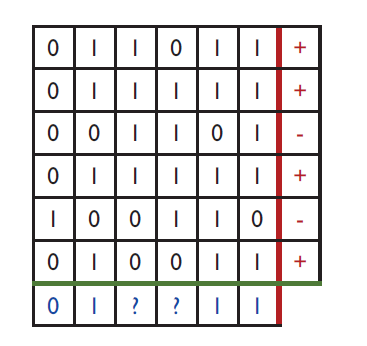
\includegraphics[width=0.6\linewidth]{6DL/figures/Boolean.png}
		\caption{Boolean literals}
		\label{Boolean literals}
	\end{figure}
	
	\noindent Figure: Each of the first six rows of the table represents a training example with
	its label, $+$ or $-$, indicated in the last column. The last row contains $0$(respectively
	1)in column if the $ith$ entry is $0$(respectively 1) for all the positive examples
	It contains $"?"$ if both $0$ and $1$ appear as an $ith$ entry for some positive example
	Thus, for this training sample, the hypothesis returned by the consistent algorithm
	described in the text is $\bar{x_1}\wedge x_2 \wedge x_5 \wedge x_6$.
\end{example}
\begin{example}[Universal concept class]
	Consider $\mathcal{X}=\{0,1\}^n$, of all Boolean vectors with n components, $\mathcal{Y}=\{positive, negative\}$, and $\mathcal{H}$ be the function class of all functions from $\mathcal{X}$ to $\mathcal{Y}$. Is this fucntion class PAC-learnable?
	To guarantee a consistent hypothesis the hypothesis class must include all the fucntions. Since $|\mathcal{H}|=2^{(2^n)}$. Theorem 9 gives the following sample complexity bound:
	\begin{equation}
	m>\frac{1}{\epsilon}\left((\log2)2^n+\log\frac{1}{\delta}\right)
	\end{equation}
	Here, the number of training samples required is exponential in $n$, which is the cost
	of the representation of a point in $\mathcal{X}$. Thus, PAC-learning is not guaranteed by
	the theorem.
\end{example}

\subsection{Guarantees for finite hypothesis sets-inconsistent case}
In the most general case, there may be no hypothesis in $\mathcal{H}$ consistent with the labeled training sample. This, in fact, is the typical case in practice, where the learning problems may be somewhat difficult or the concept classes more complex than the hypothesis set used by the learning algorithm. However, inconsistent hypotheses with a small number of errors on the training sample can be useful and as we shall see, can benefit from favorable guarantees under some assumptions. This section presents learning guarantees precisely for this inconsistent case and finite hypothesis sets.\\
To derive learning guarantees in this more general setting, we will use Hoeffding's inequality or the following corollary, which relates the generalization error and empirical error of a single hypothesis.

\begin{corollary}
	Fix $\epsilon > 0$ and let $S$ denote an i.i.d sample of size $m$. Then for any $h$ mapping  from $\mathcal{X}$ to $\{0,1\}$, the following inequalities hold:
	\begin{align}
	& P_{S\sim D^m} (\hat{R}_S (h)-R(h) \geq \epsilon) \leq \exp(-2m\epsilon^2)\\
	& P_{S\sim D^m} (\hat{R}_S (h)-R(h) \leq-\epsilon) \leq \exp(-2m\epsilon^2)\\
	& P_{S\sim D^m} (|\hat{R}_S (h)-R(h)| \geq \epsilon) \leq 2\exp(-2m\epsilon^2)
	\end{align}
	\begin{proof}
		The results follows immediately by Hoeffding's inequality.
	\end{proof}
\end{corollary}

\begin{corollary}[Generalization bound-single hypothesis]
	Fix a hypothesis $h$ mapping  from $\mathcal{X}$ to $\{0,1\}$. Then for any $\delta > 0$, the following inequality holds with probability at least $1-\delta$:
	$$R(h) \leq \hat{R}_S(h) + \sqrt{\frac{\log \frac{1}{\delta}}{2m}}$$
\end{corollary}
\begin{proof}
	Setting the right-hand side of (2.16) to be equal to $\delta$ and solving for $\epsilon$ yields immediately the bound.
\end{proof}
\noindent This is more general but not as tight as the previous one since it does not utilize the fact $\hat{R}_S(h)=0$.\\
\begin{example}[Tossing a coin]
	Imagine tossing a biased coin that lands heads with probability $p$, and let our
	hypothesis be the one that always guesses heads. Then the true error rate is $R(h)=p$
	and the empirical error rate $\hat{R}(h)=\hat{p}$ where $\hat{p}$ is the empirical probability of heads based on the training sample drawn i.i.d. Thus, corollary 6 guarantees with
	probability at least $1-\delta$ that
	\begin{equation}
	|p-\hat{p}| \leq \sqrt{\frac{\log\frac{2}{\delta}}{2m}}
	\end{equation}
	Therefore, if we choose $\delta=0.02$ and use a sample of size $500$, with probability at
	least $98\%$, the following approximation quality is guaranteed for $\hat{p}$:
	\begin{equation}
	|p-\hat{p}| \leq \sqrt{\frac{\log(10)}{1000}} \approx 0.048
	\end{equation}
\end{example}

Although the result of Corollary 6 is very simple, it has very limited practical meaning. The main reason is that it only applies to a single fixed function h. Essentially, it says that for each fixed function $h$, there is a set $\mathcal{S}$ of samples(whose measure $P(\mathcal{S}) \geq 1-\delta$) for all $S\in \mathcal{S}$, $|\hat{R}_S(h)-R(h)|$ is bounded. However, such $\mathcal{S}$ sets could be different for different functions.
Thus, as in the proof for the consistent case, we need to derive a uniform convergence bound, that is a bound that holds with high probability for all hypotheses $h \in \mathcal{H}$. since:
\begin{equation}
\hat{R}_S(\hat{h}_S)-R_S(\hat{h}_S) \leq \sup_{h \in \mathcal{H}}(\hat{R}_S(h)-R(h))
\end{equation}
We proceed to explain how one can obtain uniform bounds.\\

\begin{theorem}[Learning bound-finite $\mathcal{H}$, inconsistent case]
	Let $\mathcal{H}$ be a finite hypothesis set. Then, for any $\delta>0$ with probability at least $1-\delta$ the following inequality holds:
	$$\forall h \in \mathcal{H}, \quad |R(h) - \hat{R}_S(h)| \leq \sqrt{\frac{\log |\mathcal{H}| + \log \frac{2}{\delta}}{2m}}$$
\end{theorem}

\begin{proof}
	\begin{align}
	P\left( \exists h \in \mathcal{H}: |\hat{R}_S (h)-R(h)| \geq \epsilon \right)
	&= P\left(\bigcup_{h \in \mathcal{H}} \{ |\hat{R}_S (h)-R(h)| \geq \epsilon \} \right) \\
	(Union\ bound)&\leq \sum_{h \in \mathcal{H}} P\left( |\hat{R}_S (h)-R(h)| \geq \epsilon \right) \\
	&\leq 2|H|\exp(-2m\epsilon^2)      	
	\end{align}
	Setting the right-hand side to be equal to $\delta$ completes the proof.
\end{proof}

Since this is a uniform upper bound, it can be applied to $\hat{h}_S$, as (14) says. \\

Thus for finite hypothesis set $\mathcal{H}$,
\begin{equation}
R(h) \leq \hat{R}_S(h) + O\left( \sqrt{\frac{\log |\mathcal{H}|}{2m}} \right)
\end{equation}

Note that the bound suggests seeking a trade-off between reducing the empirical error versus controlling the size of the hypothesis set: a larger hypothesis set is penalized by the second term but could help reduce the empirical error, that is the first term. But, for a similar empirical error, it suggests using a smaller hypothesis set.\\


Also note that we could also bound the expected value of $\mathbb{E}[\sup_{h \in \mathcal{H}} |R(h)-\hat{R}_S(h)|]$ by using the fact that for any nonnegative random variable $Z$, $\mathbb{E}[Z] = \int_{0}^{\infty} P(Z>t)dt$.

From the above PAC learning examples we can see that
\begin{itemize}
	\item It requires assumptions on data generation, i.e. samples are i.i.d.
	\item The error bounds are valid with respect to repeated samples of training data.
	\item For a fixed function we roughly have $|R(h)-\hat{R}_S(h)| \approx \frac{1}{\sqrt{m}}$.
	\item If $\mathcal{H}=n$ then $\sup_{h \in \mathcal{H}} |R(h)-\hat{R}_S(h)| \approx \sqrt{\frac{\log n}{m}}$. The term $\log n$ can be thought as the complexity of the hypothesis space $\mathcal{H}$.
\end{itemize}

There are several things which can be improved.
\begin{itemize}
	\item 	Hoeffding's inequality does not utlize the variance information. So the results could be improved by
	utilizing such information.
	\item The union bound could be quite loose. For instance, it is as bad as if all the functions in $\mathcal{H}$ were independent.
	\item 	The supremum over $\mathcal{H}$ might be too conservative.
\end{itemize}

The bound in Example 2 becomes meaningless when $n$ is infinite. The following example generalizes it to the case of coutably many classifiers.

\begin{corollary}[countable number of classifiers]
	Consider the case $\mathcal{H}=\{h_1,h_2,...,h_n,...\}$. Since we
	need to bound the probability of the set of misleading samples (which could mislead any $h\in \mathcal{H}$ by $\delta$, we
	need budget the proability of being misled by $h_n$ to $\omega_n\delta$ such that $\sum_{k=1}^{\infty} \omega_k \leq 1$. So in order to apply the lemma, $\epsilon$ must be chosen related to $h \in \mathcal{H}$, which is: 
	\begin{equation}
	P\left( \exists k \in \mathbb{N}: R(h_k)- \hat{R}_S (h_k) \geq \epsilon_k \right) \leq \delta
	\end{equation}
	we only need to make sure that for any k,
	\begin{equation}
	P\left( R(h_k)- \hat{R}_S (h_k) \geq \epsilon_k \right) \leq \omega_k\delta
	\end{equation}
	Since,
	\begin{align}
	P\left( \exists k \in \mathbb{N}: R(h_k)- \hat{R}_S (h_k) \geq \epsilon_k \right) &= P\left( \bigcup_{k=1}^{\infty} \{R(h_k)- \hat{R}_S (h_k) \geq \epsilon_k \} \right) \\
	&\leq \sum_{k=1}^{\infty} P\left( R(h_k)- \hat{R}_S (h_k) \geq \epsilon_k \right) \\
	&= \sum_{k=1}^{\infty} \omega_k\delta \\
	&\leq \delta
	\end{align}
	Again the first inequality comes from the Bonferroni inequality. By a similar argument, we solve $\epsilon_k$ by setting
	$\exp(-2m\epsilon_k^2)= \omega_k\delta$ which leads to $\epsilon_k = \sqrt{\frac{1}{2m} \log\frac{1}{\omega_k\delta}}$. Thus we have with probability $(1-\delta)$,
	\begin{equation}
	\forall k \in \mathbb{N}, R(h_k) \leq \hat{R}_S(h_k)+ \sqrt{\frac{\log \frac{1}{\omega_k}+ \log \frac{1}{\delta}}{2m}} 
	\end{equation}
\end{corollary}

Note that the statement is probabilistic over the the samples drawn, so that the $\omega_k$'s can not depend upon the samples drawn. This means $\omega_k$'s have to be specified before seeing the training data, otherwise the result will not hold. One
way to interpret $\omega_k$'s is that they can be thought as the "prior" knowledge about the functions(such as in Bayesian inference), which means that if you had some prior guess as to which predictors are likely be the ERM predictor (of course this guess can not depend on the data), then you should choose these values of $\omega_k$'s to be large in the theorem.\\

\section{Infinite Hypothesis Class}
\subsection{Growth Function And VC Dimension}
We have considered the case when $\mathcal{H}$ is finite or countably infinite. In practice, however, the function class
$\mathcal{H}$ could be uncountable. Under this situation, the previous method does not work. The key idea is to group
functions based on the sample
Given a sample $S=\{(x_1,y_1),..,(x_n,y_n)\}$, Consider the set
$$\mathcal{H}_{x_1,...,x_n} = \{(h(x_1),...,h(x_n)) : h\in \mathcal{H}\} $$
The size of this set is the total number of possible ways that $(x_1,...,x_n)$ can be classified. For binary classification the cardinality of this set is always finite, no matter how large $\mathcal{H}$ is.
\begin{definition}[Growth Function]
	The growth function is the macimum number of wags into which n points
	can be classified by the function class:
	$$G_\mathcal{H}(n) = \sup_{\{x_1,...,x_n\} \in \mathcal{X}^n} |\mathcal{H}_{x_1,...,x_n}|$$
\end{definition}
\noindent Growth function can be thought as a measure of the "size" for the class of functions $\mathcal{H}$. Several facts about the growth function:
\begin{itemize}
	\item When $\mathcal{H}$ is finite, we always have $G_\mathcal{H}(n) \leq |\mathcal{H}|=m$
	\item 	Since $h(x)\in \{0,1\}$, we have $G_\mathcal{H}(n) \leq2^n$. If $G_\mathcal{H}(n) =2^n$, then there is a set of $n$ points such that the class of functions $\mathcal{H}$ can generate any possible classification result on these points.
\end{itemize}	
\begin{definition}[Shatterring]
	We say that $\mathcal{H}$ shatters $\{x_1,...,x_n\}$ if $|\mathcal{H}_{x_1,...,x_n}|=2^n$
\end{definition}
\begin{definition}[VC Dimension]
	The VC dimension of a class $\mathcal{H}$ is the cardinality of the largest set that can be shattered by $\mathcal{H}$:
	$$dim_{VC}(\mathcal{H})= \sup\{n : G_\mathcal{H}(n)=2^n\}$$
\end{definition}
Note that, by definition, if $dim_{VC}(\mathcal{H})=d$, there exists a set of size $d$ that can
be fully shattered. But, this does not imply that all sets of size $d$ or less are fully
shattered, in fact, this is typically not the case.\\
To further illustrate this notion, we will examine a series of examples of hypothesis
sets and will determine the VC-dimension in each case. To compute the VC dimension we will typically show a lower bound for its value and then a matching upper bound. To give a lower bound $d$ for $dim_{VC}(\mathcal{H})$, it suffices to show that a set $S$ of cardinality $d$ can be shattered by $\mathcal{H}$. To give an upper bound, we need to prove that no set $S$ of cardinality $d+1$ can be shattered by $\mathcal{H}$, which is typically more difficult.\\
\begin{example}
	Consider all functions of the form $\mathcal{H}=\{h(x)=I(x\leq \theta), \theta \in \mathbb{R}\}$. Then it can shatter 2 points, but for any three points it cannot shatter. So the VC dimension in this case is 2.
\end{example}
\begin{example}
	Consider all linear classifiers in $\mathbb{R}^2$. In this case, all linear classifiers can
	shatter a set of 3 points. No set of four points can be shattered by linear classifiers. So the VC dimension of the hyperplanes in $\mathbb{R}^2$ is 3.
\end{example}
\begin{example}
	Consider all linear classifiers in a p-dimensional Euclidean space, i.e. $\mathcal{X}=\mathbb{R}^p$. Given $x_1,...,x_n \in \mathbb{R}^p$, we define the augmented data vector:\\
	$$z_i=[1,x_i]^T \in \mathbb{R}^{p+1}, i=1,...,n $$
	Then the set of all linear classifiers can be written as
	$$H=\{h:h(z)=sgn(\theta^Tz),\theta\in \mathbb{R}^{p+1}\}$$
	Define
	$$Z=[z_1,...,z_n] \in \mathbb{R}^{(p+1)\times n}$$
	and we argue that $x_1,...x_n$ is shattered by $\mathcal{H}$ if and only if the n columns of Z are linearly independent.
	\begin{itemize}
		\item If columns $z_1,...,z_n$ are linearly independent, we have $n<p+1$ and for any possible classification assignment $y \in \{\pm1\}^n$ the linear system $Z^T \theta=y$ must have a solution. Thus, there is a linear classifier in $\mathcal{H}$ (by taking the solution of the linear equation) which can produce such arbitrary class assignment $y$. Thus $x_1,...,x_n$ can be shattered by $\mathcal{H}$.
		\item Suppose $x_1,...,x_n$ are shattered by $\mathcal{H}$. 
		This means that for each classification $y\in \{\pm1\}^n$, there exists a 
		$\theta_y\in \mathbb{R}^{d+1}$ such that $sgn(\theta_y\cdot x_i) = y_i$. It follows that the range of the matrix
		$Z^T$ intersects every quadrant in $\mathbb{R}^n$. This implies that the matrix $Z^T$ has full rank (i.e. its
		range must be all of $\mathbb{R}^n$) and thus the columns of $Z$ are linearly independent.
	\end{itemize}
	Since if $n>p+1$ it is not possible to have $Z$'s columns linearly independent, but for $n<p+1$ we can always find such $x_1,...x_n$ to make it happen, we have $dim_{VC}(\mathcal{H})=p+1$.
\end{example}
A somewhat surprising result shows that the growth function $G_{\mathcal{H}}$ either grows exponentially in $n$ or only increases polynomially in $n$, depends on whether $n$ is greater than its VC dimension or not.
\begin{theorem}[Sauer]
	If $\mathcal{H}$ is a class of functions with binary outputs and its VC dimension is $d=dim_{VC}(\mathcal{H})$, Then for all $n \in \mathbb{N}$,
	\begin{equation}
	G_\mathcal{H}(n) \leq \sum_{i=0}^{d}\binom{n}{i}
	\end{equation}
\end{theorem}
\begin{proof}
 We prove this by induction on $d$ and $n$. 
 
 For the base case, we note that if $n \leq d$, the statement of the theorem is vacuously true, and if $d = 0$,
 it is clear that $\mathcal{H}$ consists of a single classification function and thus the theorem holds as well.
 
 Now assume that $n > d > 0$. Let $x_1,...,x_n\in \mathcal{X}$ be an arbitrary set of points. Consider the following
 two subsets of $\{\pm1\}^{n-1}$.
 \begin{equation}
  S_1 = \{y\in \{\pm 1\}^{n-1}:\exists h\in \mathcal{H}~\text{s.t.}~y_i = h(x_i),~i = 1,...,n-1\} 
 \end{equation}
  \begin{equation}
  S_2 = \{y\in \{\pm 1\}^{n-1}:\exists h_1, h_2\in \mathcal{H}~\text{s.t.}~y_i = h_1(x_i) = h_2(x_i),~h_1(x_n) = 1,~h_2(x_n) = -1\} 
 \end{equation}
 Here $S_1$ is the set of classifications which occur for $x_1,...,x_{n-1}$ and $S_2$ is the set of 
 classifications of $x_1,...,x_{n-1}$ for which $x_n$ can be either $\pm 1$. It is clear that
 \begin{equation}
  |\mathcal{H}_{x_1,...,x_n}| = |S_1| + |S_2|
 \end{equation}
 since $S_1$ is the set of classifications of the first $n-1$ points which occur and $S_2$ is the set of classifications
 of the first $n-1$ points which occur twice (once with $x_n = 1$ and once with $x_n = -1$). Moreover, at most $d$ points
 can be shattered by $S_1$ and at most $d-1$ points can be shattered by $S_2$ since $\mathcal{H}$ shatters at most $d$ points
 (any points shattered by $S_2$ would be shattered together with $x_n$ by $\mathcal{H}$). The inductive hypothesis then implies
 that
 \begin{equation}
  |S_1| \leq \sum_{i=0}^{d}\binom{n-1}{i},~|S_2| = \sum_{i=0}^{d-1}\binom{n-1}{i}
 \end{equation}
 Thus we get
 \begin{equation}
  |\mathcal{H}_{x_1,...,x_n}| = |S_1| + |S_2| \leq \sum_{i=0}^{d}\binom{n-1}{i} + \binom{n-1}{i-1} = \sum_{i=0}^{d}\binom{n}{i}
 \end{equation}
 Since $x_1,...,x_n$ were arbitrary points, we see that
 \begin{equation}
  G_\mathcal{H}(n) \leq \sum_{i=0}^{d}\binom{n}{i}
 \end{equation}
 as desired.
\end{proof}
From this, we deduce the following polynomial bound in $n$.
\begin{corollary}
	Let $\mathcal{H}$ be a hypothesis set with $dim_{VC}(\mathcal{H})=d$. Then for all $n\geq d $,
	\begin{equation}
	G_\mathcal{H}(n) \leq \left(\frac{en}{d} \right)^d = O(n^d)
	\end{equation}
\end{corollary}
\begin{proof}
	The proof begins by using Sauers lemma.
	\begin{align}
	G_\mathcal{H}(n) &\leq \sum_{i=0}^{d}\binom{n}{i} \\
	&\leq \left(\frac{n}{d}\right)^d \sum_{i=0}^{d}\binom{n}{i} \left(\frac{d}{n}\right)^i \\
	&\leq \left(\frac{n}{d}\right)^d \sum_{i=0}^{n}\binom{n}{i} \left(\frac{d}{n}\right)^i \\
	&= \left(\frac{n}{d}\right)^d \left(1+ \frac{d}{n}\right)^n \\
	&\leq \left(\frac{en}{d}\right)^d
	\end{align}
\end{proof}

\subsection{Generalization Bound For Binary Classification}
We introduce the generalization error bound which utilizes the growth function of $\mathcal{H}$ or VC dimension of $\mathcal{H}$ instead of the naive cardinality $|\mathcal{H}|$. Recall that we are trying to determine how fast
\begin{equation}
\mathbb{P}_{(X_1,Y_1),...,(X_n,Y_n)} \left(\sup_{h \in \mathcal{H}}|\hat{R}(h)-R(h)|>\epsilon \right)
\end{equation}
decays as $n\to \infty$. We are also assuming that the loss function $\ell$ is bounded
The problem when the set $\mathcal{H}$ is finite is covered in the notes, it is simply an
application of the union bound. The famous trick which solves the problem
when $\mathcal{H}$ is uncountably infinite is called the symmetrization lemma. In order to
simplify notation,I will denote by $S = \{(X_1,Y_1),...,(X_n,Y_n) \}$ the random data samples.
\begin{lemma}[Symmetrization lemma]
	Let $\epsilon_1,...,\epsilon_n$ be iid random variables which take the values $\pm1$ each with probability $\frac{1}{2}$ (i.e. random signs) and let $\Phi : \mathbb{R}\to \mathbb{R}$ be a convex function. Then
	\begin{equation}
	\mathbb{E}_S\Phi\left(\sup_{h \in \mathcal{H}}|\hat{R}(h)-R(h)| \right) \leq 2\mathbb{E}_S\mathbb{E}_{\epsilon_1,...,\epsilon_n} \Phi \left(\sup_{h \in \mathcal{H}} \frac{1}{n} \bigg|\sum_{i=1}^{n}\epsilon_i \ell(y_i,h(x_i))\bigg| \right)
	\end{equation}
\end{lemma}

\begin{proof}
	The proof proceeds by rewriting the expectation as follows
	\begin{equation}
	\mathbb{E}_S\Phi\left(\sup_{h \in \mathcal{H}}|\hat{R}(h)-R(h)| \right)=\mathbb{E}_S\Phi\left(\sup_{h \in \mathcal{H}}\frac{1}{n} \bigg|\sum_{i=1}^{n}\epsilon_i \ell(y_i,h(x_i))-\mathbb{E}_{(X'_i,Y'_i)} \ell(y'_i,h(x'_i))\bigg| \right)
	\end{equation}
	where $(X'_i,Y'_i)$ are i.i.d. with distribution $(X,Y)$. This formula holds because by definition
	\begin{equation}
	\mathbb{E}_{(X'_i,Y'_i)} \ell(y'_i,h(x'_i)) = R(h)
	\end{equation}
	The$(x'_i,y'_i)$ are called ghost samples. We can rewrite the above as
	\begin{equation}
	\mathbb{E}_S\Phi\left(\sup_{h \in \mathcal{H}}|\hat{R}(h)-R(h)| \right)=\mathbb{E}_S\Phi\left(\sup_{h \in \mathcal{H}}\frac{1}{n} \bigg|\mathbb{E}_{S'} \sum_{i=1}^{n}\epsilon_i \ell(y_i,h(x_i))-\ell(y'_i,h(x'_i)) \bigg| \right)
	\end{equation}
	where $S'$ represents the distribution of the ghost samples. By the triangle
	inequality, we can pull the expectation out of the absolute value to get
	\begin{equation}
	\mathbb{E}_S\Phi\left(\sup_{h \in \mathcal{H}}|\hat{R}(h)-R(h)| \right) \leq \mathbb{E}_S\Phi\left(\sup_{h \in \mathcal{H}} \mathbb{E}_{S'} \frac{1}{n} \bigg| \sum_{i=1}^{n}\epsilon_i \ell(y_i,h(x_i))-\ell(y'_i,h(x'_i)) \bigg| \right)
	\end{equation}
	We can also pull the expectation out of the supremum. If you wish, this can be
	viewed as an application of Jensen's inequality(or the triangle inequality, which follows from Jensen's inequality). Again by Jensen's inequality we can move the expectation outside of $\Phi$(since $\Phi$ is assumed to be convex). This yields
	\begin{equation}
	\mathbb{E}_S\Phi\left(\sup_{h \in \mathcal{H}}|\hat{R}(h)-R(h)| \right) \leq \mathbb{E}_S\mathbb{E}_{S'}\Phi\left(\sup_{h \in \mathcal{H}} \frac{1}{n} \bigg| \sum_{i=1}^{n}\epsilon_i \ell(y_i,h(x_i))-\ell(y'_i,h(x'_i)) \bigg| \right)
	\end{equation}
	Now comes the incredible trick. We observe the following symmetry between $S$ and $S'$. All of the samples in $S$ and $S'$ are iid with the same distribution! This means that we can swap the i-th sample in $S$ with the i-th sample in $S'$ and the distribution of both, and thus the expectation, remain	unchanged. Furthermore, this swapping can be done for any subset of indices $\{i_1,...,i_k\}$, and the expectation still remains unchanged.
	
	We now choose a uniformly random subset of indices, perform this swapping
	for the subset, and take the expectation over the random subset. Since the value
	of the left-hand side above is independent of where we swapped, we will get the same value
	
	We now note that if the i-th sample in $S$ and $S'$ are swapped, then this
	has the effect of negating the term
	\begin{equation}
	\ell(y_i,h(x_i))-\ell(y'_i,h(x'_i))
	\end{equation}
	This means that the random swapping procedure described above is the same
	as negating each term in the sum independently with probability $\frac{1}{2}$. Putting
	this together, we see that the left hand side above is equal to
	\begin{equation}
	\mathbb{E}_{\epsilon_1,...,\epsilon_n}\mathbb{E}_{S,S'} \Phi\left(\sup_{h \in \mathcal{H}} \frac{1}{n} \bigg| \sum_{i=1}^{n}\epsilon_i (\ell(y_i,h(x_i))-\ell(y'_i,h(x'_i))) \bigg| \right)
	\end{equation}
	where the $\epsilon_i$ are random signs ($\pm1$ with probability $\frac{1}{2}$).
	Finally, we rewrite this as
	\begin{equation}
	\mathbb{E}_{\epsilon_1,...,\epsilon_n}\mathbb{E}_{S,S'} \Phi\left(\sup_{h \in \mathcal{H}} \frac{1}{n} \bigg| \sum_{i=1}^{n}\epsilon_i \ell(y_i,h(x_i))- \sum_{i=1}^{n}\epsilon_i\ell(y'_i,h(x'_i)) \bigg| \right)
	\end{equation}
	and use the triangle inequality and the convexity of $\Phi$ in combination with the
	fact that $S$ and $S'$ are identically distributed to get
	\begin{equation}
	\mathbb{E}_S\Phi\left(\sup_{h \in \mathcal{H}}|\hat{R}(h)-R(h)| \right) \leq \mathbb{E}_{S}\mathbb{E}_{\epsilon_1,...,\epsilon_n} \Phi \left(2\sup_{h \in \mathcal{H}} \frac{1}{n} \bigg| \sum_{i=1}^{n}\epsilon_i (\ell(y_i,h(x_i))\bigg| \right)
	\end{equation}
	as desired.
\end{proof}
Suppose now that the function $\Phi$ is convex and non-decreasing on $[0,\infty]$.
The important point of this lemma is that the random signs $\epsilon_i$ are independent
of the sample! This permits us to use the union bound in combination with the
growth function of the function class $\mathcal{H}$ to obtain
\begin{equation}
\mathbb{E}_{\epsilon_1,...,\epsilon_n} \Phi \left(2\sup_{h \in \mathcal{H}} \frac{1}{n} \bigg| \sum_{i=1}^{n}\epsilon_i (\ell(y_i,h(x_i))\bigg| \right) \leq G_{\mathcal{H}}(n) \sup_{h \in \mathcal{H}_S} \mathbb{E}_{\epsilon_1,...,\epsilon_n} \Phi \left( \frac{2}{n} \bigg| \sum_{i=1}^{n}\epsilon_i (\ell(y_i,h(x_i))\bigg| \right)
\end{equation}
We can now choose $\Phi$ appropriately to estimate $\mathbb{P}_S \left(\sup_{h \in \mathcal{H}}|\hat{R}(h)-R(h)|>\epsilon \right)$.
For instance, we choose
\begin{numcases}{\Phi(x)=}
0, & $x\leq \frac{\epsilon}{2}$ \\
\frac{2}{\epsilon}(x-\frac{\epsilon}{2}), & $x> \frac{\epsilon}{2}$
\end{numcases}
Then we have that
\begin{equation}
\mathbb{P}_S \left(\sup_{h \in \mathcal{H}}|\hat{R}(h)-R(h)|>\epsilon \right) \leq \mathbb{E}_S \Phi \left(\sup_{h \in \mathcal{H}}|\hat{R}(h)-R(h)| \right)
\end{equation}
and we proceed to estimate
\begin{equation}
\mathbb{E}_{\epsilon_1,...,\epsilon_n} \Phi \left( \frac{2}{n} \bigg| \sum_{i=1}^{n}\epsilon_i (\ell(y_i,h(x_i))\bigg| \right)
\end{equation}
using Hoeffding's inequality. First we have
\begin{equation}
\mathbb{E}_{\epsilon_1,...,\epsilon_n} \Phi \left( \frac{2}{n} \bigg| \sum_{i=1}^{n}\epsilon_i (\ell(y_i,h(x_i))\bigg| \right) = \frac{2}{\epsilon} \int_{\frac{\epsilon}{2}}^{\infty} \mathbb{P}_{\epsilon_1,...,\epsilon_n} \left( \frac{2}{n} \bigg| \sum_{i=1}^{n}\epsilon_i (\ell(y_i,h(x_i))\bigg| >\lambda \right) d\lambda
\end{equation}
Hoeffding's inequality now implies that
\begin{equation}
\mathbb{P}_{\epsilon_1,...,\epsilon_n} \left( \frac{2}{n} \bigg| \sum_{i=1}^{n}\epsilon_i (\ell(y_i,h(x_i))\bigg| >\lambda \right) \leq 2\exp \left(-\frac{n\lambda^2}{8} \right)
\end{equation}
and then change variables to get
\begin{equation}
\mathbb{E}_{\epsilon_1,...,\epsilon_n} \Phi \left( \frac{2}{n} \bigg| \sum_{i=1}^{n}\epsilon_i (\ell(y_i,h(x_i))\bigg| \right) \leq \frac{4}{\epsilon}\sqrt{\frac{8}{n}} \int_{\frac{\epsilon}{2}\sqrt{\frac{n}{8}}}^{\infty} \exp(-\tau^2) d\tau
\end{equation}
By bounding the Gaussian tail integral, we will obtain a bound of the form 
\begin{equation}
\int_{x}^{\infty} \exp(-\tau^2) d\tau \leq \frac{\exp(-x^2)}{2x}
\end{equation}
which gives
\begin{equation}
\mathbb{E}_{\epsilon_1,...,\epsilon_n} \Phi \left( \frac{2}{n} \bigg| \sum_{i=1}^{n}\epsilon_i (\ell(y_i,h(x_i))\bigg| \right) \leq \frac{32}{n\epsilon^2} \exp\left(-\frac{n\epsilon^2}{32} \right)
\end{equation}
and then we get
\begin{equation}
\mathbb{P}_S \left(\sup_{h \in \mathcal{H}}|\hat{R}(h)-R(h)|>\epsilon \right) \leq G_{\mathcal{H}}(n) \frac{32}{n\epsilon^2} \exp\left(-\frac{n\epsilon^2}{32} \right)
\end{equation}
Now observe that
\begin{equation}
\min\{1,\frac{\exp(-x)}{x}\} \leq 2\exp(-x)
\end{equation}
Replace $x$ by $\frac{32}{n\epsilon^2}$, so we finally get 
\begin{equation}
\mathbb{P}_S \left(\sup_{h \in \mathcal{H}}|\hat{R}(h)-R(h)|>\epsilon \right) \leq 2G_{\mathcal{H}}(n) \exp\left(-\frac{n\epsilon^2}{32} \right)
\end{equation}
We have already proved the Vapnik-Chervonenkis theorem below.
\begin{theorem}[Growth function generalization bound]
	Let $\mathcal{H}$ be a family of functions taking values from $\{+1, -1\}$. Then for any $\delta>0$, with probability at least $1-\delta$, we have
	\begin{equation}
	\forall h \in \mathcal{H}, R(h) \leq \hat{R}(h)+ 4\sqrt{\frac{2\log(2G_{\mathcal{H}}(n))+2\log\frac{2}{\delta}}{n}}
	\end{equation}
\end{theorem}
\begin{proof}
	Setting $\delta = 2G_{\mathcal{H}}(n) \exp\left(-\frac{n\epsilon^2}{32} \right)$ and solve $\epsilon$ we have the result.
\end{proof}
The explicit relationship just formulated between VC-dimension and the growth
function combined with the corollary of Sauer leamma leads immediately to the following generalization bounds based on the VC-dimension.
\begin{corollary}[VC-dimension generalization bound]
	Let $\mathcal{H}$ be a family of functions taking values from $\{+1, -1\}$ with VC-dimension $d_{\mathcal{H}}$. Then for any $\delta>0$, with probability at least $1-\delta$, we have
	\begin{equation}
	\forall h \in \mathcal{H}, R(h) \leq \hat{R}(h)+ 4\sqrt{\frac{2d_{\mathcal{H}}\log(\frac{en}{d_{\mathcal{H}}})+2\log\frac{4}{\delta}}{n}}
	\end{equation}
\end{corollary}
\begin{proof}
	Sauer lemma implies that $	G_\mathcal{H}(n) \leq \left(\frac{en}{d} \right) ^d$, and then by replacing $G_\mathcal{H}(n)$ by the term $\left(\frac{en}{d}\right) ^d$ in Theorem 9 we got this VC-dimension generalization bound. 
\end{proof}
Moreover, integrating the tail distribution bound one can obtain a bound on the expectation
\begin{align}
\mathbb{E}_S \left(\sup_{h \in \mathcal{H}}|\hat{R}(h)-R(h)| \right) &= \int_{0}^{\infty}  \mathbb{P}_S \left(\sup_{h \in \mathcal{H}}|\hat{R}(h)-R(h)|>\epsilon \right) d\epsilon \\
&\leq \int_{0}^{\infty} 2G_{\mathcal{H}}(n)\exp\left(-\frac{n\epsilon^2}{32} \right)d\epsilon\\
&=G_{\mathcal{H}}(n) \sqrt{\frac{32\pi}{n}}
\end{align}
However this bound doesn't make sense, since $G_{\mathcal{H}}(n)$ grows polynomially in $n$. We use another trick to obtain a bound on the expectation that makes snese.\\
For simplicity, we denote $Z=\sup_{h \in \mathcal{H}}|\hat{R}(h)-R(h)|$.
\begin{align}
\mathbb{E}[Z^2] &= \int_{0}^{\infty} \mathbb{P}(Z^2\geq \epsilon) d\epsilon \\
& = \int_{0}^{u} \mathbb{P}(Z^2\geq \epsilon) d\epsilon + \int_{u}^{\infty} \mathbb{P}(Z^2\geq \epsilon) d\epsilon \\
& \leq u+    \int_{u}^{\infty} 2G_{\mathcal{H}}(n) \exp\left(-\frac{n\epsilon}{32} \right) d\epsilon \\
& = u+\frac{64G_{\mathcal{H}}(n)}{n}\exp \left(-\frac{nu}{32}\right)
\end{align}
Minimizing the RHS respect to $u$ we have $u=\frac{32\log(2G_{\mathcal{H}}(n))}{n}$. Plugging in we have $\mathbb{E}[Z^2] \leq \frac{32\log(8G_{\mathcal{H}}(n))}{n}$.
By the Cauchy-Schwarz inequality we have 
\begin{equation}
\mathbb{E}_S \left(\sup_{h \in \mathcal{H}}|\hat{R}(h)-R(h)| \right)= \mathbb{E}[Z] \leq \sqrt{\mathbb{E}[Z^2]} \leq \sqrt{\frac{32\log(8G_{\mathcal{H}}(n))}{n}}
\end{equation}

\subsection{Natarajan-dimension and Natarajan's lemma}
There is a natural way to generalize the VC-dimension to the  non-binary functions case. A naive attempt is to simply generalize the definition of shattering, that we say $\mathcal{H}$ shatters $S \subset \mathcal{X}$, if $\mathcal{H}|_{S} = \mathcal{Y}^{S}$. However, this condition is too strong that will not lead to tight bounds on the hypothesis set complexity. For example, in the non-binary case, we take the hypothesis set $\mathcal{H}$ to be $\mathcal{H} = (\mathcal{Y} \backslash \{l_0\})^{\mathcal{X}}$, which means $\mathcal{H}$ only leave the label $l_0$ out but includes every function else. In this case, $\mathcal{H}$ is capable to classify while it is dimension is $0$ which is unresonable. 

Forgetting this naive definition, we recall two alternative generalizations, introduced by \textbf{Natarajan(1989)}. In both definition, we reduce the requirement of shattering, which only needs $\mathcal{H}$ contains a function whose behavior on $T$ differs from its behavior on $S\backslash T$, where $T$ and $S\backslash T$ is any partition of $S$. The two dimensions differ in how "different behavior" is defined.
\begin{definition}[Graph dimension]
	Let $\mathcal{H} \subset \mathcal{Y}^{\mathcal{X}}$ be a hypothesis set and let $S \subset \mathcal{X}$. We say that $\mathcal{H}$ G-shatters $S$ if there exists an $f: S\to \mathcal{Y}$ such that for every $T\subset S$, there is a $g \in \mathcal{H}$ such that
	\begin{equation}
	\forall x \in T, g(x)=f(x), \quad and \quad \forall x \in S\backslash T, g(x)\ne f(x).
	\end{equation}
	The graph dimension of $\mathcal{H}$, denoted by $d_G(\mathcal{H})$, is the maximal cardinality of a set that is G-shattered by $\mathcal{H}$. More precisely:
	\begin{equation}
	d_G(\mathcal{H}) = \sup \{|S| : S \subset \mathcal{X} \text{ is G-shatterd by } \mathcal{H}\}
	\end{equation} 
\end{definition}

\begin{definition}[Natarajan dimension]
	Let $\mathcal{H} \subset \mathcal{Y}^{\mathcal{X}}$ be a hypothesis set and let $S \subset \mathcal{X}$. We say that $\mathcal{H}$ N-shatters $S$ if there exists $f_1, f_2 : S\to \mathcal{Y}$ such that $\forall y \in S, f_1(y)\ne f_2(y)$, and for every $T\subset S$, there is a $g \in \mathcal{H}$ such that
	\begin{equation}
	\forall x \in T, g(x)=f_1(x), \quad and \quad \forall x \in S\backslash T, g(x)=f_2(x).
	\end{equation}
	The Natarajan dimension of $\mathcal{H}$, denoted by $d_N(\mathcal{H})$, is the maximal cardinality of a set that is N-shattered by $\mathcal{H}$. More precisely:
	\begin{equation}
	d_N(\mathcal{H}) = \sup \{|S| : S \subset \mathcal{X} \text{ is N-shatterd by } \mathcal{H}\}
	\end{equation} 
\end{definition}
Both of these two dimensions coincide with the VC-dimension for binary case when $|\mathcal{Y}|=2$. So they are generalizations of VC-dimension. Note that we always have $d_N  \leq d_G$.

By the way, in Ben David et al.(1995), it was proved that for every function class $\mathcal{H}\subset \mathcal{Y}^{\mathcal{X}}$,
\begin{equation}
d_N(\mathcal{H}) \leq d_G(\mathcal{H}) \leq 4.67 \log_2(|\mathcal{Y}|)d_N(\mathcal{H})
\end{equation}
which implies that, when the label sapce $\mathcal{Y}$ is finite (exactly the case we care about), the Natarajan dimension and the Graph dimension are equivalent, just with a constant difference. Since $d_N  \leq d_G$, we will use Natarajan dimension to bound the generalization error. 

The significance of introducing the Natarajan dimension lies in that we can obtain a relatively tight generalization bound in multi-classification case. First we need to bound the growth function in terms of Natarajan dimension. Similarly as the Sauer Lemma, we have the following combinatorial result: 

\begin{lemma}[From Natarajan 1988b]
	Let $X$ and $Y$ be two finite sets, and $H \subset Y^{X}$, If $k$ is the size of the ;argest subset of $X$ N-shattered by $H$, then we have:
	\begin{equation}
	|H| \leq (|X|)^k (|Y|)^{2k}
	\end{equation}
\end{lemma}
\begin{proof}
	By induction on $|X|$.
	It is clearly true for $|X|=1$, for all $|Y|$. Assume true for $|X|=l$, $|Y|= m$, and prove for $|X|=l+1$, $|Y|= m$. Let $X= \{x_1,...,x_{l+1}\}$ and $Y=\{y_1,...,y_l\}$. Define the subsets $|H_i|$ of $|H|$ as follows:
	\begin{equation}
	H_i := \{f| f\in H, f(x_1)=y_i \}
	\end{equation}
	Also, for $i\ne j$ define the sets of functions $H_{ij}(i\ne j)$ and $H_0$ as follows:
	\begin{equation}
	H_{ij} := \{f| f\in H_i, \exists g \in H_j \text{ such that } f=g \text{ on } X-\{x_1\} \}
	\end{equation}
	\begin{equation}
	H_0 := H - \bigcup_{i\ne j} H_{ij}
	\end{equation}
	Now we have
	\begin{equation}
	|H| = |H_0| + |\cup_{i\ne j}H_{ij}| \leq |H_0| + \sum_{i\ne j}|H_{ij}|
	\end{equation}
	we seek bounds on the quantities on the right-hand side of the last inequality. By
	definition, the functions in $H_0$ are all distinct on the m elements of $X \backslash \{x_1\}$. So that $H_0$ can be viewed as function class restricted on $X \backslash \{x_1\}$ which has $l$ elements.
	Furthermore, the largest set shattered in $H_0$ must be of cardinality no greater than
	$k$. Hence, we have by the inductive hypothesis,
	\begin{equation}
	|H_0| \leq l^km^{2k}
	\end{equation}
	and then, we claim that every $H_{ij}$ shatters a set of cardinality at most $k-1$. Otherwise, assume that it shatters $k$ ponits. By definition $H$ would shatter the $k$ points plus $x_1$, which is a set of cardinality greater than $k$. A contradiction. Also  since the functions in H are all distinct on $X \backslash \{x_1\}$, we have by the inductive hypothesis, for $i\ne j$
	\begin{equation}
	|H_{ij}| \leq l^{k-1}m^{2(k-1)}
	\end{equation}
	Combining the last three inequalities, we have
	\begin{align}
	|H| &\leq l^km^{2k} + \sum_{i\ne j}l^{k-1}m^{2(k-1)} \\
	&\leq l^km^{2k} + m^2l^{k-1}m^{2(k-1)} \\ 
	&= l^{k-1}m^{2k}(l+1) \\
	&\leq (l+1)^km^{2k}
	\end{align}
	By induction, we completes the proof.
\end{proof}

\begin{corollary}\label{cor3.1}
	For any input space $\mathcal{X}$, any finite label space $\mathcal{Y}$ $(|\mathcal{Y}|< \infty)$ and any $\mathcal{H} \subset \mathcal{Y}^{\mathcal{X}}$, The Natarajan dimension of $\mathcal{H}$ is denoted by $d_N$, then for any $n>0$,
	\begin{equation}
	G_{\mathcal{H}}(n) \leq n^{d_N}|\mathcal{Y}|^{2d_N}
	\end{equation}
\end{corollary}
\begin{proof}
	By definition of growth function, there exist $S\subset \mathcal{X}$, $|S|=n$, such that $	G_{\mathcal{H}}(n)= |\mathcal{H}|_S|$.
	
	For $\mathcal{H}|_S \subset \mathcal{Y}^S$, use the lemma to get $|\mathcal{H}|_S| \leq |S|^k|\mathcal{Y}|^{2k}$, where $k$ is the Natarajan dimension of $\mathcal{H}|_S$. Of course $k\leq d_N$. So we get
	\begin{equation}
	G_{\mathcal{H}}(n)= |\mathcal{H}|_S| \leq |S|^k|\mathcal{Y}|^{2k} \leq n^{d_N}|\mathcal{Y}|^{2d_N}
	\end{equation}
\end{proof}
\subsection{Generalization bounds for multi-classification}
After obtaining the bound of growth function under multi-classification assumptions, actually we have already proved one of the main results of this paper.

\begin{theorem}[Natarajan-dimension generalization bounds]
	Let $\mathcal{H}$ be a family of functions taking values from $\{1,2,...,k\}$ with Natarajan-dimension $d_N$ and assume that the loss function $\ell$ is the 0-1 loss. $S$ is the sample set with size $n$. Then for any $\delta>0$, with probability at least $1-\delta$, we have
	\begin{equation}
	\forall h \in \mathcal{H}, R(h) \leq \hat{R}_S(h)+4\sqrt{\frac{2d_N\log(k^2n)+2\log\frac{4}{\delta}}{n}}
	\end{equation}
\end{theorem}
\begin{proof}
	The relationship between Natarajan-dimension and the growth function showed in Corollary\ref{cor3.1} combined with Theorem\ref{th3} leads immediately to the generalization bounds based on Natarajan-dimension.
\end{proof}

\section{Rademacher Complexity}
\subsection{Rademacher complexity bounds}
In the previous section, we have talked about the growth function and the VC-dimension and obtain the genralization bound based on these two complexity. In this section, we introduce a different notion of complexity for the family of hypotheses, Rademacher complexity. This will help us derive learning guarantees using relatively simple proofs based on McDiarmid's inequality, while obtaining high-quality bounds.

We will continue to use $\mathcal{H}$ to denote a hypothesis set as in the previous chapters
and $h$ an element of $\mathcal{H}$. Many of the results of this section are general and hold for
an arbitrary loss function $\ell :\mathcal{Y}\times \mathcal{Y} \to \mathbb{R}$. To each $h: \mathcal{X}\to \mathcal{Y}$ , we can associate a function $g$ that maps $(x,y)$ to $\ell(h(x),y)$ without explicitly describing the specific loss $\ell$ used. In what follows $G$ will generally be interpreted as the family of loss functions associated to $\mathcal{H}$.

The Rademacher complexity captures the richness of a family of functions by
measuring the degree to which a hypothesis set can fit random noise. The following
states the formal definitions of the empirical and average Rademacher complexity.
\begin{definition}[Empirical Rademacher complexity]
	Let $g$ be a family of functions mapping from $Z$ to $[a,b]$ and $S=(z_1,...,z_m)$ a fixed
	sample of size m with elements in $Z$. Then, the empirical Rademacher complexity
	of G with respect to the sample $S$ is defined as:
	\begin{equation}
	\hat{\mathcal{R}}_S(G)= \mathbb{E}_{\sigma} \big[\sup_{g\in G}\frac{1}{m}\sum_{i=1}^{m}\sigma_ig(z_i)\big]
	\end{equation}
	where $\sigma=(\sigma_1,...,\sigma_m)^T$ with $\sigma_i$s independent uniform random variables taking values in $\{+1,-1\}$. The random variables $\sigma_i$ are called Rademacher variables
\end{definition}
The empirical Rademacher complexity measures on average how well the function class G correlates with random noise on $S$. This describes the richness of the family $G$. Richer or more complex families $G$ can generate more vectors $(g(z_1),...,g(z_m))$ and thus better correlate with random noise on average.
\begin{definition}[Rademacher complexity]
	Let $D$ denote the distribution according to which samples are drawn. For any
	integer $m \geq 1$, the Rademacher complexity of $G$ is the expectation of the empirical
	Rademacher complexity over all samples of size $m$ draw according to $D$
	\begin{equation}
	\mathcal{R}_m(G)= \mathbb{E}_{S\sim D^m}[\hat{\mathcal{R}}_S(G)]
	\end{equation}
\end{definition}
We are now ready to present our first generalization bounds based on Rademacher complexity.
\begin{theorem}
	Let G be a family of functions mapping from $Z$ to $[0,1]$. Then, for any $\delta>0$, with
	probability at least $1-\delta$, each of the following holds for all $g\in G$
\end{theorem}
\begin{equation}
\mathbb{E}[g(z)] \leq \frac{1}{m}\sum_{i=1}^{m}g(z_i) +2\mathcal{R}_m(G) +\sqrt{\frac{\log(\frac{1}{\delta})}{2m}}
\end{equation}
\begin{equation}
and \qquad	\mathbb{E}[g(z)] \leq \frac{1}{m}\sum_{i=1}^{m}g(z_i) +2\hat{\mathcal{R}}_S(G) +3\sqrt{\frac{\log(\frac{2}{\delta})}{2m}}
\end{equation}
\begin{proof}
	For any sample $S=(z_1,...z_m)$ and any $g\in G$, we denote by $\hat{\mathbb{E}}_S[g]$ the empirical average of $g$ over $S$: $\hat{\mathbb{E}}_S[g]= \frac{1}{m} \sum_{i=1}^{m}g(z_i)$. We define $\Phi$ for any sample $S$ and then apply the McDiarmid's inequality
	\begin{equation}
	\Phi(S)= \sup_{g\in G}(\mathbb{E}[g]-\hat{\mathbb{E}}_S[g])
	\end{equation}
	Let $S$ and $S'$ be two samples differing by exactly one point, say $z_m$ in $S$ and $z_m'$ in $S'$. Then we have
	\begin{align}
	\Phi(S')-\Phi(S) &= \sup_{g\in G}(\mathbb{E}[g]-\hat{\mathbb{E}}_{S'}[g]) -\sup_{g\in G}(\mathbb{E}[g]-\hat{\mathbb{E}}_S[g])\\
	&\leq \sup_{g\in G}(\hat{\mathbb{E}}_S[g])-\hat{\mathbb{E}}_{S'}[g])\\
	&= \sup_{g\in G} \frac{g(z_m)-g(z'_m)}{m} \\
	&\leq \frac{1}{m}
	\end{align}
	Similarly, we can obtain $\Phi(S)-\Phi(S')\leq \frac{1}{m}$, thus $|\Phi(S')-\Phi(S)|\leq \frac{1}{m}$. Then, by McDiarmid's inequality, for any $\delta>0$, with probability at least $1-\frac{2}{\delta}$, the following holds
	\begin{equation}
	\Phi(S)\leq \mathbb{E}_S[\Phi(S)]+ \sqrt{\frac{\log(\frac{1}{\delta})}{2m}}
	\end{equation}
	Next we will show $\mathbb{E}_S[\Phi(S)] \leq 2\mathcal{R}_m(G)$
	\begin{align}
	\mathbb{E}_S[\Phi(S)]&= \mathbb{E}_S\bigg[\sup_{g\in G}(\mathbb{E}[g]-\hat{\mathbb{E}}_S[g])\bigg]\\
	&=\mathbb{E}_S\bigg[\sup_{g\in G}\mathbb{E}_{S'}\big[\hat{\mathbb{E}}_{S'}[g]-\hat{\mathbb{E}}_S[g]\big]\bigg]\\
	&\leq \mathbb{E}_{S,S'}\bigg[\sup_{g\in G}(\hat{\mathbb{E}}_{S'}[g]-\hat{\mathbb{E}}_S[g])\bigg]\\
	&= \mathbb{E}_{S,S'}\bigg[\sup_{g\in G}\frac{1}{m}\sum_{i=1}^{m}(g(z'_i)-g(z_i))\bigg]\\
	&= \mathbb{E}_{\sigma,S,S'}\bigg[\sup_{g\in G}\frac{1}{m}\sum_{i=1}^{m}\sigma_i(g(z_i)-g(z'_i))\bigg]\\
	&\leq  \mathbb{E}_{\sigma,S'}\bigg[\sup_{g\in G}\frac{1}{m}\sum_{i=1}^{m}\sigma_ig(z'_i)\bigg] + \mathbb{E}_{\sigma,S}\bigg[\sup_{g\in G}\frac{1}{m}\sum_{i=1}^{m}-\sigma_ig(z_i)\bigg]\\
	&\leq 2\mathbb{E}_{\sigma,S}\bigg[\sup_{g\in G}\frac{1}{m}\sum_{i=1}^{m}\sigma_ig(z_i)\bigg] = 2\mathcal{R}_m(G)
	\end{align}
	The reduction to $\mathcal{R}_m(G)$ yields the bound in the first inequality, using $\delta$ instead of $\frac{\delta}{2}$. To derive a bound in terms of $\hat{\mathcal{R}}_S(G)$, we observe that, changing one point in $S$ changes $\hat{\mathcal{R}}_S(G)$ by at most $\frac{1}{m}$. Then
	using again McDiarmid's inequality, with probability $1-\frac{\delta}{2}$ the following holds
	\begin{equation}
	\mathcal{R}_m(G)\leq \hat{\mathcal{R}}_S(G) +\sqrt{\frac{\log(\frac{2}{\delta})}{2m}}
	\end{equation}
	Finally, we use the union bound to combine these two inequalities which yield that
	with probability at least $1-\delta$
	\begin{equation}
	\Phi(S) \leq 2\hat{\mathcal{R}}_S(G)+3\sqrt{\frac{\log(\frac{2}{\delta})}{2m}}
	\end{equation}
\end{proof}

The following result relates the empirical Rademacher complexities of a hypothesis set $h$ and to the family of loss functions $G$ associated to $\mathcal{H}$ in the case of binary loss(0-1 loss)
\begin{lemma}
	Let $\mathcal{H}$ be a family of functions taking values in $\mathcal{Y}=\{+1,-1\}$, and let $G$ be the family of loss functions associated to $\mathcal{H}$ for the 0-1 loss:$G=\{(x,y) \mapsto 1_{h(x)\ne y} | h\in \mathcal{H}\}$.
	For any sample $S=\{(x_1, y1),..., (x_m, y_m)\}$, let $S_{\mathcal{X}}$ denote its projection over $S_{\mathcal{X}}=(x_1,.., x_m)$. Then, the following relation holds
	between the Rademacher complexities of $G$ and $\mathcal{H}$:
	\begin{equation}
	\mathcal{R}_m(G)=\frac{1}{2} \mathcal{R}_m(\mathcal{H})
	\end{equation}
\end{lemma}
\begin{proof}
	\begin{align}
	\hat{\mathcal{R}}_S(G)&= \mathbb{E}_{\sigma} \big[\sup_{h\in \mathcal{H}}\frac{1}{m}\sum_{i=1}^{m}\sigma_i1_{h(x)\ne y}\big]\\
	&=\mathbb{E}_{\sigma} \big[\sup_{h\in \mathcal{H}}\frac{1}{m}\sum_{i=1}^{m}\sigma_i\frac{1}{2}(1-y_ih(x_i))\big]\\
	&= \frac{1}{2} \mathbb{E}_{\sigma} \big[\sup_{h\in \mathcal{H}}\frac{1}{m}\sum_{i=1}^{m}\sigma_i y_ih(x_i)\big] = \frac{1}{2}\hat{\mathcal{R}}_{S_{\mathcal{X}}}(\mathcal{H})
	\end{align}
	Taking expectation on both sides over $S$ concludes the lemma.
\end{proof}
These connections between the empirical and average Rademacher complexities can be used to derive generalization bounds for binary classification in terms of the Rademacher complexities of the hypothesis set $\mathcal{H}$.
\begin{theorem}[Rademacher complexity bounds for binary classification]
	Let $\mathcal{H}$ be a family of functions taking values in $\mathcal{Y}=\{+1,-1\}$, and let $F$ be the distribution over the input space $\mathcal{X}$. Then, for any $\delta>0$, with probability at least $1-\delta$ over a sample $S$ of size $m$ drawn according to $F$, each of the following holds for all $h\in \mathcal{H}$:
	\begin{equation}
	\qquad R(h) \leq \hat{R}(h) + \mathcal{R}_m(\mathcal{H}) + \sqrt{\frac{\log(\frac{1}{\delta})}{2m}}
	\end{equation}
	\begin{equation}
	and \qquad R(h) \leq \hat{R}(h) + \hat{\mathcal{R}}_{S}(\mathcal{H}) + 3\sqrt{\frac{\log(\frac{2}{\delta})}{2m}}
	\end{equation}
\end{theorem}
\begin{proof}
	The result follows immediately by theorem 3. 1 and lemma 3.1
\end{proof}
%%%
%
%
%
%
%
%
%
%
%
%
%
%
%
%
The theorem provides two generalization bounds for binary classification based on the Rademacher complexity. Note that the second bound, (3.18), is data-dependent. Thus, this bound could be particularly informative if we could compute $\hat{\mathcal{R}}_{S}(\mathcal{H})$.
For binary classification problem, the empirical Rademacher complexity $\hat{\mathcal{R}}_{S}(\mathcal{H})$ can actually be computed. Notice that:
\begin{align}
\hat{\mathcal{R}}_{S}(\mathcal{H}) &= \mathbb{E}_{\sigma} \big[\sup_{h\in \mathcal{H}}\frac{1}{m}\sum_{i=1}^{m}\sigma_i h(x_i)\big]\\
&= 1+2\mathbb{E}_{\sigma} \big[\sup_{h\in \mathcal{H}}\frac{1}{m}\sum_{i=1}^{m}-\frac{1-\sigma_i h(x_i)}{2}\big]\\
&= 1-2\mathbb{E}_{\sigma} \big[\inf_{h\in \mathcal{H}}\frac{1}{m}\sum_{i=1}^{m} \frac{1-\sigma_i h(x_i)}{2}\big]\\
&= 1-2\mathbb{E}_{\sigma} \big[\inf_{h\in \mathcal{H}}\frac{1}{m}\sum_{i=1}^{m} 1_{h(x_i)\ne \sigma_i} \big] \\
&= 1-2\mathbb{E}_{\sigma} \big[\inf_{h\in \mathcal{H}}\hat{R}_S(h,\sigma)\big]
\end{align}

where $\hat{R}_S(h,\sigma)$ is the empirical risk of classifier $h$ with respect to $S$ with random label $\sigma=(\sigma_1,...,\sigma_m)$. When $\mathcal{H}$ is so large that it can fit every random labeling perfectly, we have $\hat{\mathcal{R}}_{S}(\mathcal{H})=1$ and the bound becomes meaningless.\\

We could estimate Rademacher complexity for function classes which are built from simpler classes. The following is a list of properties about Rademacher complexity.
\begin{itemize}
	\item 1. If $\mathcal{F}\subset \mathcal{G}$ then $\mathcal{R}_m(\mathcal{F}) \leq \mathcal{R}_m(\mathcal{G})$. It follows from the definition.
	\item 2. $\mathcal{R}_m(c\cdot \mathcal{F}) = |c|\mathcal{R}_m(\mathcal{F})$, where $c\cdot \mathcal{F}=\{x\mapsto cf(x) | f\in \mathcal{F}\}$. Since we have 
	\begin{equation}
	\mathcal{R}_m(c\cdot \mathcal{F})= \mathbb{E}_{\sigma,S}\bigg[\sup_{f\in \mathcal{F}}\frac{1}{m}\sum_{i=1}^{m}c\sigma_i f(x_i)\bigg] = \mathbb{E}_{\sigma,S}\bigg[|c|\sup_{f\in \mathcal{F}}\frac{1}{m}\sum_{i=1}^{m}\sigma_i f(x_i)\bigg] = |c|\mathcal{R}_m(\mathcal{F})
	\end{equation}
	\item 3. $\mathcal{R}_m(\mathcal{F}+g) = \mathcal{R}_m(\mathcal{F})$, where $\mathcal{F}+g$ is defined as $\{f+g| f\in \mathcal{F}\}$ and $g$ is a fixed function. To show this we have:
	\begin{align}
	\mathcal{R}_m(\mathcal{F}+g) &= \mathbb{E}_{\sigma,S}\bigg[\sup_{f\in \mathcal{F}}\frac{1}{m}\sum_{i=1}^{m}\sigma_i (f(x_i)+g(x_i))\bigg]\\
	&= \mathbb{E}_{\sigma,S}\bigg[\sup_{f\in \mathcal{F}}\frac{1}{m}\sum_{i=1}^{m}\sigma_i f(x_i)\bigg] + \mathbb{E}_{\sigma,S}\bigg[\frac{1}{m}\sum_{i=1}^{m}\sigma_i g(x_i)\bigg]\\
	&=\mathcal{R}_m(\mathcal{F})
	\end{align}
	\item 4. Let the convex hull of a set of functions $\mathcal{F}$ be defined as
	\begin{equation}
	conv(\mathcal{F}) = \left\{ \sum_{i=1}^{k}\alpha_if_i : k\geq 1,\alpha_i\geq 0, \sum_{i=1}^{k}\alpha_i=1, f_1,...,f_k\in \mathcal{F} \right\}.
	\end{equation}
	Then we have $\mathcal{R}_m(\mathcal{F})= \mathcal{R}_m(conv(\mathcal{F}))$ since
	\begin{align}
	\mathcal{R}_m(conv(\mathcal{F})) &= \mathbb{E}\bigg[ \sup_{f_j\in \mathcal{F}, \alpha_i\geq 0, \sum_{i=1}^{k}\alpha_i=1} \frac{1}{m} \sum_{i=1}^{m}\sigma_i \sum_{j=1}^{k} \alpha_jf_j(x_i) \bigg]\\
	&= \mathbb{E}\bigg[ \sup_{f_j\in \mathcal{F}, \alpha_i\geq 0, \sum_{i=1}^{k}\alpha_i=1}\sum_{j=1}^{k}\alpha_j \left( \frac{1}{m} \sum_{i=1}^{m}\sigma_i  f_j(x_i) \right) \bigg]\\
	&= \mathbb{E}\bigg[ \sup_{f_j\in \mathcal{F}}\max_{j} \frac{1}{m}\sum_{i=1}^{m}\sigma_if_j(x_i) \bigg]\\
	&= \mathcal{R}_m(\mathcal{F})
	\end{align}
\end{itemize}
The Rademacher complexity is related to the growth funciton and VC-dimension. In the next sections, we will bound the Rademacher complexity by the growth funciton and VC-dimension which are easier to compute.
\subsection{The relation between Rademacher complexity and VC dimension}
First we will show how the Rademacher complexity can be bounded in terms of growth function. We will use Massart's lemma.
\begin{theorem}[Massart's lemma]
	Let $A \subset {\mathbb{R}}^m$ be a finite set, with $r=\max_{x\in A}||x||_2$, then the following holds:
	\begin{equation}
	\mathbb{E}_{\sigma} \big[\frac{1}{m}\sup_{x\in A}\sum_{i=1}^{m}\sigma_ix_i\big] \leq \frac{r\sqrt{2\log|A|}}{m}
	\end{equation}
	where $\sigma_i's$ are independent uniform random variables taking values in $\{-1,+1\}$ and $x_1,...,x_m$ are components of vector $x$.
\end{theorem}
\begin{proof}
	For any $t>0$, using Jensen's inequality, rearranging terms, and bounding the supremum by a sum, the independence of the $\sigma_i's$, and Hoeffding's lemma, we obtain:
	\begin{align}
	\exp\left(t\mathbb{E}_{\sigma} \big[\sup_{x\in A}\sum_{i=1}^{m}\sigma_ix_i \big]\right) &\leq \mathbb{E}_{\sigma}\left( \exp \left(t\sup_{x\in A}\sum_{i=1}^{m}\sigma_ix_i\right)\right) \\
	&= \mathbb{E}_{\sigma}\left(\sup_{x\in A} \exp \left(t\sum_{i=1}^{m}\sigma_ix_i\right)\right)\\
	&\leq \sum_{x\in A} \mathbb{E}_{\sigma}\left(\exp \left(t\sum_{i=1}^{m}\sigma_ix_i\right)\right)\\
	(\text{independence of the }\sigma_i's)&=\sum_{x\in A} \prod_{i=1}^{m}\mathbb{E}_{\sigma_i}[\exp(t\sigma_ix_i)] \\
	(\text{Hoeffding's lemma})&\leq \sum_{x\in A} \prod_{i=1}^{m} \exp\left(\frac{t^2(2x_i)^2}{8}\right)\\
	&= \sum_{x\in A}\exp\left(\frac{t^2||x||_2^2}{2}\right)\\
	&\leq  \sum_{x\in A} \exp\left(\frac{t^2r^2}{2}\right) = |A|\exp\left(\frac{t^2r^2}{2}\right)
	\end{align}
	Taking the log of both sides and dividing by t gives us:
	\begin{equation}
	\mathbb{E}_{\sigma} \big[\sup_{x\in A}\sum_{i=1}^{m}\sigma_ix_i \big] \leq \frac{\log|A|}{t} + \frac{tr^2}{2}
	\end{equation}
	Minimizes RHS, when $t=\frac{\sqrt{2\log|A|}}{r}$ we get:
	\begin{equation}
	\mathbb{E}_{\sigma} \big[\sup_{x\in A}\sum_{i=1}^{m}\sigma_ix_i \big] \leq r\sqrt{2\log|A|}
	\end{equation}
	Dividing both sides by $m$ leads to the statement of the lemma.
\end{proof}
Using this result, we can now bound the Rademacher complexity in terms of the growth function.
\begin{corollary}
	Let $G$ be a family of functions taking values in $\{-1,+1\}$. Then the following holds
	\begin{equation}
	\mathcal{R}_m(G) \leq \sqrt{\frac{2\log G_G(m)}{m}}
	\end{equation}
\end{corollary}
\begin{proof}
	For a fixed sample $S=(x_1,...,x_m)$, we denote by $G_S$ the set of vectors of function values $(g(x_1),...,g(x_m))$ where $g \in G$. Since $g$ takes values in $\{-1,+1\}$, the norm of these vectors is bounded by $\sqrt{m}$. We can then apply Massart's lemma as follows:
	\begin{equation}
	\mathcal{R}_m(G)= \mathbb{E}_{S}\bigg[\mathbb{E}_{\sigma}\bigg[\sup_{u\in G_S}\frac{1}{m}\sum_{i=1}^{m}\sigma_iu_i\bigg]\bigg] \leq \mathbb{E}_{S}\bigg[\frac{\sqrt{m}\sqrt{2\log|G_S|}}{m} \bigg]
	\end{equation}
	By definition, $|G_S|$ is bounded by the growth function, thus
	\begin{equation}
	\mathcal{R}_m(G) \leq \mathbb{E}_{S}\bigg[\frac{\sqrt{m}\sqrt{2\log G_G(m)}}{m} \bigg] =\sqrt{ \frac{2\log G_G(m)}{m}}
	\end{equation}
	which concludes the proof.
\end{proof}
Combining the generalization bound of Rademacher complexity with this corollary yields immediately the following generalization bound in terms of the growth function.
\begin{corollary}[Growth function generalization bound]
	Let $\mathcal{H}$ be a family of functions taking values in $\{-1,+1\}$. Then, for any $\delta >0$, with probability at least $1-\delta$, for any $h \in \mathcal{H}$,
	\begin{align}
	R(h)&\leq \hat{R}(h) + \sqrt{\frac{2\log G_{\mathcal{H}}(m)}{m}} +\sqrt{\frac{\log\frac{1}{\delta}}{2m}}\\
	&\leq \hat{R}(h) + \sqrt{\frac{4\log G_{\mathcal{H}}(m)+\log\frac{1}{\delta}}{m}}
	\end{align}
\end{corollary}
Similarly, we can bound the growth foucntion with the VC dimension of $\mathcal{H}$ and obtain the VC dimension generalization bound.
Using Rademacher complexity is another way of getting the growth foucntion or the VC dimension generalization bound, which only differs by constants from the result we got in the previous section.\\
Another application of introducing Rademacher comlexity is to derive margin-based generalization bound in binary and multi-class case. In the next sections, we will talk about the margin based results.

\subsection{Margin based generalization bound for binary classification}
Usually we do not minimize the 0-1 loss in practice, for 0-1 loss can not gives the sense of degree to classified correctly or incorrectly. Thus the hypothesis functions of the classifier are generally mapped to the real number space, such as the linear classifier. Hyperplane was used as the basis of classification. So there is a natural measure of classification confidence, which is the directed distance between the sample point $(x_i, y_i)$ and the hyperplane $wx+b=0$, says $y_i(wx_i+b)$. The distance is greater than zero means classified correctly, and the greater the directional distance is, the greater of confidence we will have, which should correspond to a smaller loss, and vice versa. \\

Linear functions are not the only option. Generally we denote that $\mathcal{H}$ is a set of functions mapping $\mathcal{X}$ to $\mathcal{Y}' = \mathbb{R}$, and for $h \in \mathcal{H}$, $y_ih(x_i)$ is some kind of classification confidence. The label space $\mathcal{Y}$ still be the binary label $\{+1,-1\}$ and the loss function we definded to be the following margin loss. 
The quantity $\rho > 0$ should thus be interpreted as the margin we wish to acheive.

\begin{definition}[Margin Loss Function]
	For any $\rho > 0$, we define the $\rho$-margin loss $\ell_{\rho} : \mathbb{R} \times \mathbb{R} \to \mathbb{R}_{+}$ to be the function $\ell_{\rho}(y,y') = \Phi_{\rho}(yy')$ with,
	\begin{numcases}{\Phi_{\rho}(x)=}
	0 &if $\rho \leq x$ \\
	1-\frac{x}{\rho} & if $0\leq x \leq \rho$ \\
	1 & if $x \leq 0$
	\end{numcases}
\end{definition}
The margin loss function is illustrated in the figure below.
\begin{figure}[ht]    \centering 
	\begin{tikzpicture}
	% draw the axis
	\draw[-latex] (-2.5,0) -- (3,0) node[below] {$x$};
	\draw[-latex] (0,0) -- (0,2) node[above] {$y$};
	%draw node
	\foreach \x in {0,1}{\draw(\x,0)--(\x,0.05)node[below,outer sep=2pt,font=\tiny]at(\x,0){\x};}
	\foreach \y in {1}{\draw(0,\y)--(0.05, \y)node[above left, inner sep=2pt,font=\tiny]at(0,\y){\y};}
	\draw(0.6,0)--(0.6,0.05)node[below,outer sep=2pt,font=\tiny]at(0.6,0){$\rho$};
	% draw the function (piecewise)
	
	\draw[color=red, thick, smooth] (-2.5,1) -- (0,1) -- (0.6,0) -- (2.8,0);
	\draw[color=blue, dashed] (-2.5,1) -- (0.6,1) -- (0.6,0) -- (2.8,0);
	\end{tikzpicture}
	\caption{The margin loss, defined with respect to margin parameter $\rho$}
\end{figure}
\\
\\
\\
\\
The empirical margin loss is then defined as the margin loss over the training sample.
\begin{definition}[Empirical Margin Loss]
	Given a sample $S=\{(x_1,y_1),..,(x_n,y_n)\}$ and hypothesis $\mathcal{H}$ a set of real-valued functions, the empirical margin loss is	defined by
	\begin{equation}
	\hat{R}_{\rho}(h) = \frac{1}{m} \sum_{i=1}^{n} 	\Phi_{\rho}(y_ih(x_i))
	\end{equation}
\end{definition}

Note that for any the empirical margin loss can be upper-bounded as follows
\begin{equation}
\hat{R}_{\rho}(h) \leq \frac{1}{m} \sum_{i=1}^{n} 1_{y_ih(x_i) \leq \rho}
\end{equation}
and $y_ih(x_i)\leq 0$ means that $(x_i, y_i)$ is classified incorrectly by $h$, so that the generalization error is 
\begin{equation}
R(h) = \mathbb{E}_{X,Y}[1_{Yh(X) \leq 0}]
\end{equation}
$y_ih(x_i)$ can be thought as some kind of confidence. $y_ih(x_i)>0$ means $h$ classify $(x_i,y_i)$ correctly, and the larger $y_ih(x_i)$ is, the more confidence we have. The upper bound of margin loss admits a simple interpretation: it is the fraction of the points in the
training sample $S$ that have been misclassified or classified with confidence less than $\rho$.

When $h$ is a linear function defined by a weight vector w with $||w||=1$, then $y_ih(x_i)$ has a explicit geometry interpretation, which is nothing but the geometry distance of the sample $(x_i,y_i)$ to the hyperplane $h(x)=0$.

The next lemma will be needed for the proof of the margin-based generalization bound.
\begin{lemma}[Talagrand's lemma]
	Let $\Phi: \mathbb{R} \to \mathbb{R}$ be an L-Lipschitz function, $S=\{(x_1,y_1),..,(x_n,y_n)\}$ be the sample set. Then, for any hypothesis set $\mathcal{H}$ of real-valued functions, the following inequality holds
	\begin{equation}
	\hat{\mathcal{R}}_S(\Phi \circ \mathcal{H}) \leq L \hat{\mathcal{R}}_S(\mathcal{H})
	\end{equation} 
\end{lemma}
\begin{proof}
	By definition, we have
	\begin{align}
	\hat{\mathcal{R}}_S(\Phi \circ \mathcal{H}) &= \frac{1}{n} \mathbb{E}_{\sigma} \bigg[\sup_{h \in \mathcal{H}} \sum_{i=1}^{n} \sigma_i(\Phi \circ h)(x_i)\bigg] \\
	&= \frac{1}{n} \mathbb{E}_{\sigma_1,...,\sigma_{n-1}} \bigg[\mathbb{E}_{\sigma_n} \big[ \sup_{h \in \mathcal{H}} u_{n-1}(h) + \sigma_n(\Phi \circ h)(x_n)\big]\bigg]
	\end{align}
	where we denote $\sum_{i=1}^{n-1} \sigma_i(\Phi \circ h)(x_i)$ by $u_{n-1}(h)$. By the definiton of supremum, for any $\epsilon>0$, there exist $h_1, h_2$ such that
	\begin{equation}
	u_{n-1}(h_1) + (\Phi \circ h_1)(x_n) \geq \sup_{h \in \mathcal{H}} \big[u_{n-1}(h) + (\Phi \circ h)(x_n)- \epsilon \big] 
	\end{equation}
	\begin{equation}
	u_{n-1}(h_2) - (\Phi \circ h_2)(x_n) \geq \sup_{h \in \mathcal{H}} \big[u_{n-1}(h) - (\Phi \circ h)(x_n)- \epsilon \big] 
	\end{equation}
	Thus, by definition of the expectation of $\mathbb{E}_{\sigma_n}$
	\begin{align}
	& \mathbb{E}_{\sigma_n} \big[ \sup_{h \in \mathcal{H}} u_{n-1}(h) + \sigma_n(\Phi \circ h)(x_n)\big] -\epsilon \\
	&= \frac{1}{2}\sup_{h \in \mathcal{H}} \big[u_{n-1}(h) + (\Phi \circ h)(x_n)  -\epsilon \big] + \frac{1}{2}\sup_{h \in \mathcal{H}} \big[u_{n-1}(h) - (\Phi \circ h)(x_n) -\epsilon \big] \\
	&\leq \frac{1}{2}\big[u_{n-1}(h_1) + (\Phi \circ h_1)(x_n)\big] +\frac{1}{2}\big[u_{n-1}(h_2) - (\Phi \circ h_2)(x_n)\big] \\
	& = \frac{1}{2}\big[u_{n-1}(h_1) + u_{n-1}(h_2) + \Phi \circ(h_1-h_2)(x_n)\big] \\
	&\leq \frac{1}{2}\big[u_{n-1}(h_1) + u_{n-1}(h_2) + L|h_1(x_n)-h_2(x_n)|\big]
	\end{align}
	Let $s=sgn(h_1(x_n)-h_2(x_n))$, then
	\begin{align}
	& \mathbb{E}_{\sigma_n} \big[ \sup_{h \in \mathcal{H}} u_{n-1}(h) + \sigma_n(\Phi \circ h)(x_n)\big] -\epsilon \\
	& \leq \frac{1}{2}\big[u_{n-1}(h_1) + sLh_1(x_n)\big] +\frac{1}{2}\big[u_{n-1}(h_2) - sLh_2(x_n)\big] \\
	&\leq  \frac{1}{2} \sup_{h \in \mathcal{H}} \big[u_{n-1}(h) + sLh(x_n)\big] +\frac{1}{2} \sup_{h \in \mathcal{H}} \big[u_{n-1}(h) - sLh(x_n)\big] \\
	&= \mathbb{E}_{\sigma_n} \big[ \sup_{h \in \mathcal{H}} u_{n-1}(h) + \sigma_n Lh(x_n)\big]
	\end{align}
	Since the inequality holds for any $\epsilon>0$, then we have
	\begin{equation}
	\mathbb{E}_{\sigma_n} \big[ \sup_{h \in \mathcal{H}} u_{n-1}(h) + \sigma_n(\Phi \circ h)(x_n)\big] \leq \mathbb{E}_{\sigma_n} \big[ \sup_{h \in \mathcal{H}} u_{n-1}(h) + \sigma_n Lh(x_n)\big]
	\end{equation}
	Proceeding in the same way for other $\sigma_i$ proves the lemma.
\end{proof}

\begin{theorem}[Margin bound for binary classification]
	Let $\mathcal{H}$ be a set of real-valued functions. Fix $\rho>0$, $S=\{(x_1,y_1),..,(x_n,y_n)\}$ be the sample set, then, for any $\delta>0$, with probability at least $1-\delta$, the following holds for all $h \in \mathcal{H}$:
	\begin{equation}
	R(h) \leq \hat{R}_{\rho}(h) + \frac{2}{\rho}\mathcal{R}_n(\mathcal{H}) + \sqrt{\frac{\log\frac{1}{\delta}}{2n}}
	\end{equation}
	\begin{equation}
	R(h) \leq \hat{R}_{\rho}(h) + \frac{2}{\rho}\hat{\mathcal{R}}_S(\mathcal{H}) + 3\sqrt{\frac{\log\frac{2}{\delta}}{2n}}
	\end{equation}
\end{theorem}
\begin{proof}
	Let $\mathcal{H}_1 = \{ z=(x,y) \mapsto yh(x) : h \in \mathcal{H} \}$ and $\mathcal{H}_2 = \{  \Phi \circ f : f \in \mathcal{H}_1 \}$. 
	Since functions in $\mathcal{H}_2$ range in $[0,1]$, by $theorem5$, with probability at least $1-\delta$, for all $g \in \mathcal{H}_2$
	\begin{equation}
	\mathbb{E}[g(z)] \leq \frac{1}{n}\sum_{i=1}^{m}g(z_i) + 2\mathcal{R}_n(\mathcal{H}_2) +\sqrt{\frac{\log\frac{1}{\delta}}{2n}}	
	\end{equation}
	Thus
	\begin{equation}
	\mathbb{E}[\Phi_{\rho}(yh(x))] \leq \hat{R}_{\rho}(h) + 2\mathcal{R}_n(\Phi_{\rho} \circ \mathcal{H}_1) +\sqrt{\frac{\log\frac{1}{\delta}}{2n}}
	\end{equation}
	Since the margin loss function is a upper bound of 0-1 loss function, we have 
	$R(h) = \mathbb{E}[1_{yh(x) \leq 0}] \leq \mathbb{E}[\Phi_{\rho}(yh(x))]$. 
	Also by the Talagrand's lemma we have $\mathcal{R}_n(\Phi_{\rho} \circ \mathcal{H}_1) \leq \frac{1}{\rho} \mathcal{R}_n(\mathcal{H}_1)$. Thus
	\begin{equation}
	R(h) \leq \hat{R}_{\rho}(h) + \frac{2}{\rho}\mathcal{R}_n(\mathcal{H}_1) +\sqrt{\frac{\log\frac{1}{\delta}}{2n}}
	\end{equation}
	And then, it is easy to show
	\begin{equation}
	\mathcal{R}_n(\mathcal{H}_1) =\frac{1}{n}\mathbb{E}_{S,\sigma}\bigg[\sup_{h \in \mathcal{H}}\sum_{i=0}^{n}\sigma_iy_ih(x_i)\bigg] = \frac{1}{n}\mathbb{E}_{S,\sigma}\bigg[\sup_{h \in \mathcal{H}}\sum_{i=0}^{n}\sigma_ih(x_i)\bigg] =  \mathcal{R}_n(\mathcal{H})
	\end{equation}
	which completes the proof of the first inequality. 
	The second inequality,(4.41), can be derived in the same way by using the second inequality of $theorem5$.
\end{proof}

To get a computable generalization bound, it is possible to bound the Rademacher complexity of linear hypotheses with bounded weight vector, as shown by the following theorem.

\begin{theorem}
	Let $\mathcal{X} = \{x \in \mathbb{R}^N: ||x|| \leq r\}$. $S \subset \mathcal{X}$ be a sample of size $n$ and let $\mathcal{H}= \{x \mapsto w \cdot x : ||w||\leq \Lambda \}$.
	Then the empirical Rademacher complexity of $\mathcal{H}$ can be bounded as follows
	\begin{equation}
	\hat{\mathcal{R}}_S(\mathcal{H}) \leq \sqrt{\frac{r^2\Lambda^2}{n}}
	\end{equation}
\end{theorem}
\begin{proof}
	Assume that $S=\{x_1,...x_n\}$.
	\begin{align}
	\hat{\mathcal{R}}_S(\mathcal{H}) &= \mathbb{E}_{\sigma}\bigg[\sup_{||w||\leq \Lambda}\frac{1}{n} \sum_{i=0}^{n}\sigma_iw \cdot x_i\bigg] \\
	\text{(Cauchy-Schwarz inequality)}&\leq \frac{\Lambda}{n}\mathbb{E}_{\sigma} ||\sum_{i=1}^{n}\sigma_ix_i||\\
	\text{(Jensens inequality)}&\leq \frac{\Lambda}{n}\bigg[ \mathbb{E}_{\sigma} ||\sum_{i=1}^{n}\sigma_ix_i||^2 \bigg]^{1/2}\\
	&= \frac{\Lambda}{n}\bigg[ \mathbb{E}_{\sigma} \big[\sum_{i,j=1}^{n}\sigma_i\sigma_j(x_i\cdot x_j) \big] \bigg]^{1/2}\\
	\text{(independent of $\sigma_i$'s)}&= \frac{\Lambda}{n}\bigg[ \sum_{i=1}^{n}||x_i||^2 \bigg]^{1/2} \\
	&\leq \frac{\Lambda}{n}\sqrt{nr^2} = \sqrt{\frac{r^2\Lambda^2}{n}}
	\end{align}
\end{proof}
Combining $theorem7$ and $theorem8$ gives directly the following general
margin bound for linear hypotheses with bounded weight vectors:
\begin{corollary}
	Assume that $\mathcal{X} = \{x \in \mathbb{R}^N: ||x|| \leq r\}$ and linear hypotheses $\mathcal{H}= \{x \mapsto w \cdot x : ||w||\leq \Lambda \}$	then, for any $\delta>0$, with probability at least $1-\delta$, for any $h\in \mathcal{H}$
	\begin{equation}
	R(h) \leq \hat{R}_{\rho}(h) + \frac{2}{\rho}\sqrt{\frac{r^2\Lambda^2}{n}} + \sqrt{\frac{\log\frac{1}{\delta}}{2n}}
	\end{equation}
\end{corollary}

This generalization bound for linear hypotheses is remarkable, since it does
not depend directly on the dimension of the feature space, but only on the margin and the radius $r$ of the sphere containing the data.
It suggests that a small generalization error can be achieved when the second term $\frac{r}{\rho}$ is small, while the first term empirical margin loss is small. The
latter occurs when few points are either classified incorrectly or correctly, but with
margin less than $\rho$.\\

The bound of the corollary gives a strong justification for margin-maximization
algorithms such as SVM. First, note that for $\rho = 1$, the margin loss can be upper
bounded by a convex function, which is called the hinge loss:
\begin{equation}
\Phi_1(x) \leq max\{1-x,0\}
\end{equation}

Using this fact, the bound of the corollary implies that with probability at least
$1-\delta$, for all $h\in \mathcal{H} = \{x \mapsto w \cdot x : ||w||\leq \Lambda \}$
\begin{equation}
R(h) \leq \frac{1}{n}\sum_{i=1}^{n}\xi_i + 2\sqrt{\frac{r^2\Lambda^2}{n}} + \sqrt{\frac{\log\frac{1}{\delta}}{2n}}
\end{equation}

where $\xi_i = max\{1-y_i(w\cdot x_i), 0\}$. The objective function minimized by the SVM
algorithm has precisely the form of this upper bound: the first term corresponds to
the slack penalty over the training set and the second to the minimization of model complexity $||w||$, which is exactly the concept of structural risk minimization. \\

As already pointed out, the bounds just discussed do not directly depend on the
dimension of the feature space and guarantee good generalization with a favorable
margin. Thus, they suggest seeking large-margin separating hyperplanes in a very
high-dimensional space. 


\subsection{Margin based generalization bound for multi classification}
For multi-class classification problem, assume that $\mathcal{Y}=\{1,2,...,k\}$. First we have a labeled sample $S=\{(x_1,y_1),...,(x_n,y_n)\} \in (\mathcal{X}\times \mathcal{Y})^n$, with $x_1,...,x_n$ drawn i.i.d. according to underlying distribution and $y_i = f(x_i)$ according to the target function $f : \mathcal{X} \to \mathcal{Y}$.

Given a classifier function $h : \mathcal{X} \to \mathcal{Y}$, with the loss function defined by 0-1 loss, the generalization error of $h$is defined as
\begin{equation}
R(h) = \mathbb{E}_{X}[1_{h(X)\ne f(X)}]
\end{equation}
To derive the margin-based generalization bounds for multi-class classification, as the binary case, we still expect to bound $R(h)$ by the margin loss $\hat{R}_{\rho}(h)$. What we need to do is generalize the definition of margin loss to multi-class case.

In the multi-class setting, a hypothesis is defined based on a scoring function $h: \mathcal{X} \times \mathcal{Y} \to \mathbb{R}$. ($h$ can also be viewed as function mapping $\mathcal{X}$ to $\mathbb{R}^\mathcal{Y}$). The label associated to point $x$ is the one resulting in the largest score $h(x, y)$:
\begin{equation}
x \mapsto \arg\max_{y\in \mathcal{Y}}h(x,y)
\end{equation}

We want the true label of $x$ obtains a high score compared to other labels. Based on this idea, we naturally define the margin $\rho_h(x, y)$ of $h$ at a sample $(x, y)$:
\begin{equation}
\rho_h(x,y) = h(x,y) - \max_{y'\ne y}h(x,y')
\end{equation}
We can see that $h$ misclassifies $(x, y)$ iff $\rho_h(x, y) \leq 0$. Thus
\begin{equation}
R(h) = \mathbb{E}_{X,Y}[1_{\rho_h(x, y) \leq 0}] 
\end{equation}
And then, for any $\rho > 0$, we can define the empirical margin loss for multi-classification as
\begin{equation}
\hat{R}_{\rho}(h) = \frac{1}{n} \sum_{i=1}^{n}\Phi_{\rho}(\rho_h(x_i, y_i))
\end{equation}  
where $\Phi_{\rho}$ is the margin loss function we defined in previous section. Similarly the empirical margin loss is upper bounded by:
\begin{equation}
\hat{R}_{\rho}(h) \leq \frac{1}{n} \sum_{i=1}^{n} 1_{\rho_h(x_i, y_i) \leq \rho}
\end{equation}
where the bound means that $(x_i,y_i)$ is misclassified by $h$ or correctly classified but with confidence less than or equal
to $\rho$.\\

First we need a lemma to derive the margin-based generalization bounds.
\begin{lemma}
	Let $\mathcal{H}_1,...,\mathcal{H}_l$ be $l$ hypothesis sets in $\mathbb{R}^{\mathcal{X}}$ and let $\mathcal{G} = \{ \max\{h_1,...,h_l\} : h_i \in \mathcal{H}_i, i=1,...,l\}$. Then, for any sample $S$ of size $n$, the empirical Rademacher complexity of $\mathcal{G}$ can be upper bounded as follows:
	\begin{equation}
	\hat{\mathcal{R}}_S(\mathcal{G}) \leq \sum_{i=1}^{l} \hat{\mathcal{R}}_S(\mathcal{H}_i)
	\end{equation}
\end{lemma}
\begin{proof}
	Let $S = (x_1,..., x_n)$. We first prove the results for $l = 2$. For any $h_1 \in \mathcal{H}_1$ and $h_2 \in \mathcal{H}_2$ we have
	\begin{equation}
	\max\{h_1, h_2\} = \frac{1}{2}[h_1 + h_2 + |h_1-h_2|]
	\end{equation}
	Thus
	\begin{align}
	\hat{\mathcal{R}}_S(\mathcal{G}) &= \frac{1}{n} \mathbb{E}_{\sigma} \bigg[\sup_{\substack{h_1 \in \mathcal{H}_1 \\ h_2 \in \mathcal{H}_2}}\sum_{i=1}^{n} \sigma_i \max\{h_1(x_i), h_2(x_i)\}\bigg] \\
	&= \frac{1}{2n} \mathbb{E}_{\sigma} \bigg[\sup_{\substack{h_1 \in \mathcal{H}_1 \\ h_2 \in \mathcal{H}_2}}\sum_{i=1}^{n} \sigma_i(h_1(x_i)+h_2(x_i)+ |h_1-h_2|(x_i))\bigg]\\
	&\leq \frac{1}{2}\hat{\mathcal{R}}_S(\mathcal{F}_1) + \frac{1}{2}\hat{\mathcal{R}}_S(\mathcal{F}_2) + \frac{1}{2n}\mathbb{E}_{\sigma} \bigg[\sup_{\substack{h_1 \in \mathcal{H}_1 \\ h_2 \in \mathcal{H}_2}}\sum_{i=1}^{n} \sigma_i|h_1-h_2|(x_i)\bigg]
	\end{align}
	Since  $x \mapsto |x|$
	is 1-Lipschitz, by Talagrand's lemma the last term can be bounded as:
	\begin{align}
	&\frac{1}{2n}\mathbb{E}_{\sigma} \bigg[\sup_{\substack{h_1 \in \mathcal{H}_1 \\ h_2 \in \mathcal{H}_2}}\sum_{i=1}^{n} \sigma_i|h_1-h_2|(x_i)\bigg] \\
	&\leq \frac{1}{2n}\mathbb{E}_{\sigma} \bigg[\sup_{\substack{h_1 \in \mathcal{H}_1 \\ h_2 \in \mathcal{H}_2}}\sum_{i=1}^{n} \sigma_i(h_1-h_2)(x_i)\bigg] \\
	&\leq \frac{1}{2n}\mathbb{E}_{\sigma} \bigg[\sup_{h_1 \in \mathcal{H}_1}\sum_{i=1}^{n} \sigma_ih_1(x_i)\bigg] + \frac{1}{2n}\mathbb{E}_{\sigma} \bigg[\sup_{h_2 \in \mathcal{H}_2}\sum_{i=1}^{n} -\sigma_ih_2(x_i)\bigg]\\
	&= \frac{1}{2}\hat{\mathcal{R}}_S(\mathcal{F}_1) + \frac{1}{2}\hat{\mathcal{R}}_S(\mathcal{F}_2)
	\end{align}
	Thus we have
	\begin{equation}
	\hat{\mathcal{R}}_S(\mathcal{G}) \leq \hat{\mathcal{R}}_S(\mathcal{F}_1) + \hat{\mathcal{R}}_S(\mathcal{F}_2)
	\end{equation}
	In general case we can write $\max\{h_1,...,h_l\}$ as $\max\{h_1, \max\{h_2,...,h_l\} \}$ and use the result of $l=2$ to constantly decrease $l$.
\end{proof}
Let $\mathcal{H} \subset \mathbb{R}^{\mathcal{X} \times \mathcal{Y}}$ be a hypothesis set, with $\mathcal{Y}=\{1,2,...,k\}$. We define:
\begin{equation}
\Pi (\mathcal{H}) = \{x\mapsto h(x,y) : h \in \mathcal{H}, y\in \mathcal{Y}\}
\end{equation}
Generalization error can be bounded by margin loss and the Rademacher complexity of $\Pi (\mathcal{H})$ we just defined. The following theorem shows this result for multi-class classification.
\begin{theorem}[Margin bound for multi-class classification]
	Fix $\rho>0$. Then, for any $\delta>0$, with probability at least $1-\delta$, the following multi-class classification generalization bound holds for all $h \in \mathcal{H}$:
	\begin{equation}
	R(h) \leq \hat{R}_\rho (h) +\frac{2k^2}{\rho} \mathcal{R}_n(\Pi_1(\mathcal{H})) + \sqrt{\frac{\log\frac{1}{\delta}}{2n}}
	\end{equation}
\end{theorem}
\begin{proof}
	The first part of the proof is similar to the binary case. Define $\mathcal{H}_1=\{(x,y)\mapsto \rho_h(x,y) : h \in \mathcal{H} \}$, $\mathcal{H}_2 = \{\Phi_{\rho}\circ f : f\in \mathcal{H}_1\}$. $\mathcal{H}_2$ take values in $[0,1]$. By $theorem5$, with probability at least $1-\delta$, for all $h \in \mathcal{H}$:
	\begin{equation}
	\mathbb{E}[\Phi_{\rho}(\rho_h(x,y))] \leq \hat{R}_\rho (h) + 2\mathcal{R}_n(\Phi_{\rho}\circ \mathcal{H}_1) + \sqrt{\frac{\log\frac{1}{\delta}}{2n}}
	\end{equation}
	Since $1_{u\leq 0} \leq \Phi_{\rho}(u)$, the generalization error is bounded by the left-hand term $R(h) = \mathbb{E}_{X,Y}[1_{\rho_h(x, y) \leq 0}] \leq \mathbb{E}[\Phi_{\rho}(\rho_h(x,y))]$.\\
	Since the $\frac{1}{\rho}$-Lipschitzness of $\Phi_{\rho}$, by Talagrand's lemma we have $\mathcal{R}_n(\Phi_{\rho}\circ \mathcal{H}_1) \leq \frac{1}{\rho} \mathcal{R}_n(\mathcal{H}_1)$. So the next part of this proof is to bound $\mathcal{R}_n(\mathcal{H}_1)$.
	\begin{align}
	\mathcal{R}_n(\mathcal{H}_1) &= \frac{1}{n} \mathbb{E}_{S,\sigma}\bigg[\sup_{h \in \mathcal{H}}\sum_{i=1}^{n}\sigma_i\rho_h(x_i,y_i)\bigg] \\
	&\leq\frac{1}{n}\sum_{y\in\mathcal{Y}}\mathbb{E}_{S,\sigma}\bigg[\sup_{h \in \mathcal{H}}\sum_{i=1}^{n}\sigma_i\rho_h(x_i,y)1_{y=y_i}\bigg]\\
	&=  \frac{1}{n}\sum_{y\in \mathcal{Y}}\mathbb{E}_{S,\sigma}\bigg[\sup_{h \in \mathcal{H}}\sum_{i=1}^{n}\sigma_i\rho_h(x_i,y)(\frac{2(1_{y=y_i})-1}{2} + \frac{1}{2}) \bigg]\\
	&\leq \frac{1}{2n}\sum_{y\in\mathcal{Y}}\mathbb{E}_{S,\sigma}\bigg[\sup_{h \in \mathcal{H}}\sum_{i=1}^{n}\sigma_i\epsilon_i \rho_h(x_i,y)\bigg] + \frac{1}{2n}\sum_{y\in\mathcal{Y}}\mathbb{E}_{S,\sigma}\bigg[\sup_{h \in \mathcal{H}}\sum_{i=1}^{n}\sigma_i \rho_h(x_i,y)\bigg]\\
	&= \frac{1}{n}\sum_{y\in\mathcal{Y}}\mathbb{E}_{S,\sigma}\bigg[\sup_{h \in \mathcal{H}}\sum_{i=1}^{n}\sigma_i \rho_h(x_i,y)\bigg]
	\end{align} 
	where $\epsilon_i=2(1_{y=y_i})-1$ and we use the fact that $\sigma_i$ and $\epsilon_i\sigma_i$ have the same distribution.\\
	Let $\Pi_1(\mathcal{H})^{(k-1)} = \{\max\{h_1,...,h_l\} : h_i \in \Pi_1(\mathcal{H}), i=1,...,k-1 \}$, and then
	\begin{align}
	\mathcal{R}_n(\mathcal{H}_1) &\leq \frac{1}{n}\sum_{y\in\mathcal{Y}}\mathbb{E}_{S,\sigma}\bigg[\sup_{h \in \mathcal{H}}\sum_{i=1}^{n}\sigma_i \big( h(x_i,y) - \max_{y'\ne y}h(x_i,y')\big)\bigg] \\
	&\leq \sum_{y\in \mathcal{Y}}\bigg[ \frac{1}{n}\mathbb{E}_{S,\sigma}\bigg[\sup_{h \in \mathcal{H}}\sum_{i=1}^{n}\sigma_i h(x_i,y)\bigg] + \frac{1}{n}\mathbb{E}_{S,\sigma}\bigg[\sup_{h \in \mathcal{H}}\sum_{i=1}^{n} \sigma_i \max_{y'\ne y}h(x_i,y')\bigg]\bigg] \\
	&\leq \sum_{y\in \mathcal{Y}}\bigg[\frac{1}{n}\mathbb{E}_{S,\sigma}\bigg[\sup_{h \in \Pi_1(\mathcal{H})}\sum_{i=1}^{n}\sigma_i h(x_i)\bigg] + \frac{1}{n}\mathbb{E}_{S,\sigma}\bigg[\sup_{h \in \Pi_1(\mathcal{H})^{(k-1)}} \sum_{i=1}^{n}\sigma_i h(x_i)\bigg]\bigg]\\
	&\leq k\bigg[\frac{k}{m} \mathbb{E}_{S,\sigma}\bigg[\sup_{h \in \Pi_1(\mathcal{H})}\sum_{i=1}^{n}\sigma_i h(x_i)\bigg]\bigg]\\
	&= k^2\mathcal{R}_n(\Pi_1(\mathcal{H}))
	\end{align}
	where the last inequality utilize the $lemma5$.
\end{proof}
For some specific hypothesis sets, a simple upper bound can be derived for the
Rademacher complexity of $\Pi_1(\mathcal{H})$, making $theorem9$ more explicit and computable. We will show this for linear hypothesis with bounded weight vectors, similarly as the binary case.\\

Assume that the samples can be represented over $\mathbb{R}^N$. In multi-class classification, the hypothesis set is based on $k$ weight vectors $w_1,...,w_k \in \mathbb{R}^N$. Each $w_i$ defines a scoring function $x \mapsto w_i\cdot x$ and the class we predict for $x \in \mathcal{X}$ is given by
\begin{equation}
\arg\max_{y\in \mathcal{Y}} w_y \cdot x
\end{equation}
We denote by $W$ the matrix formed by these weight vectors $W = (w_1,...,w_k)^T$ and we define the p-norm of $W$ by 
\begin{equation}
||W||_p = \big(\sum_{i=1}^{k}||w_i||^p\big)^{1/p}
\end{equation}
\begin{corollary}
	Let $\mathcal{X} = \{x\in\mathbb{R}^N : ||x||\leq r \} $. $\mathcal{Y}=\{1,2,...,k \} $. $S \subset \mathcal{X}$ be a sample of size $n$ and let $\mathcal{H}_p \subset \mathbb{R}^{\mathcal{X}\times \mathcal{Y}}$,
	\begin{equation}
	\mathcal{H}_p = \{(x,y) \mapsto w_y \cdot x : W = (w_1,...,w_k)^T, ||W||_p\leq \Lambda \}
	\end{equation}
	Then for any $n \geq 1$, the Rademacher complexity of $\Pi_1(\mathcal{H}_p)$ can be bounded as
	\begin{equation}
	\mathcal{R}_n(\Pi_1(\mathcal{H}_p)) \leq \sqrt{\frac{r^2\Lambda^2}{n}}
	\end{equation}
\end{corollary}
\begin{proof}
	Since $||w_i|| \leq \big(\sum_{i=1}^{k}||w_i||^p\big)^{1/p} = ||W||_p\leq \Lambda$ for all $i=1,...,k$. Thus $\Pi_1(\mathcal{H}_p) \subset \{x \mapsto w \cdot x : ||w||\leq \Lambda \}$. So the corollary is concluded by $Theorem8$.
\end{proof}

\begin{corollary}
	Assume that $\mathcal{X} = \{ x\in \mathbb{R}^N : ||x|| \leq r \}$, $\mathcal{Y}=\{1,...,k\}$ and $\mathcal{H}_p = \{(x,y) \mapsto w_y \cdot x : W = (w_1,...,w_k)^T, ||W||_p\leq \Lambda \}$, then for any $\delta >0$m with probability at least $1-\delta$, for any $h \in \mathcal{H}_p$
	\begin{equation}
	R(h) \leq \hat{R}_{\rho}(h) + \frac{2k^2}{\rho}\sqrt{\frac{r^2\Lambda^2}{n}} + \sqrt{\frac{\log\frac{1}{\delta}}{2n}}
	\end{equation}
\end{corollary}

Next, we simply describe an algorithm of \textbf{Multi-calss SVMs} that can be derived directly from the theoretical guarantees of $Corollary6$.\\
Deifine $\xi_i = \max\{1-(w_{y_i}\cdot x_i-\max_{y'\ne y_i}(w_{y'}\cdot x_i)), 0\}$, and we have for any $\delta>0$, with probability at least $1-\delta$, for all $h\in \mathcal{H}_2 = \{(x,y) \mapsto w_y \cdot x : W = (w_1,...,w_k)^T, \sum_{i=1}^{k}||w_i||^2 \leq \Lambda^2 \}$,
\begin{equation}
R(h) \leq \frac{1}{n}\sum_{i=1}^{n}\xi_i + 2k^2\sqrt{\frac{r^2\Lambda^2}{n}} + \sqrt{\frac{\log\frac{1}{\delta}}{2n}}
\end{equation}
An algorithm based on this theoretical guarantee consists of minimizing the right-hand side, that is, minimizing the empirical margin loss corresponding to the sum of the slack variables $\xi_i$, and another one minimizing $\Lambda^2$ or equivalently $\sum_{i=1}^{k}||w_i||^2$. This precisely define the multi-class SVM algorithm, which is a convex optimization problem:
\begin{align}
\min_{\xi, W} \sum_{i=1}^{n}\xi_i +& \frac{C}{2}\sum_{i=1}^{k}||w_i||^2\\
\text{subject to}\quad & \forall i=1,...,k , \forall j\ne y_i \\
&w_{y_i}\cdot x_i \geq w_j\cdot x_i +1-\xi_i
\end{align}
After we have learnd $W$, the prediction function is defined of the form $x \mapsto \arg\max_{y\in\mathcal{Y}} w_y \cdot x$.
